\documentclass[journal]{IEEEtran}

%\usepackage[brazilian]{babel}

\makeatletter
%\adddialect\l@BRAZILIAN\l@brazilian
\makeatother


\usepackage[T1]{fontenc}
\usepackage[utf8]{inputenc}
\usepackage{lmodern}

\usepackage{ae}
\usepackage{hyphenat}
\usepackage{fancyhdr}
\usepackage{float}
\usepackage{cite}
\usepackage[pdftex]{hyperref}
\usepackage[pdftex]{color,graphicx}

\usepackage[cmex10]{amsmath}
\usepackage[]{equations}
\usepackage{array}

\usepackage{mdwmath}
\usepackage{mdwtab}
\usepackage{url}
\usepackage{tikz}

\hyphenation{op-tical net-works semi-conduc-tor con-si-de-ram fa-mi-lia-ri-za-ção}
\hypersetup{colorlinks, citecolor=black, filecolor=black, linkcolor=black, urlcolor=blue}

%Algoritmos
\usepackage[english]{algorithm2e}

\begin{document}
\title{Introduction to Numeric Simulation of Magnetic Fluid Flows}

\author{Ataias~Pereira~Reis, Yuri~Dumaresq~Sobral, Francisco~Ricardo~da~Cunha\\Universidade de Brasília\\Departamento de Matemática\\Brasília, Brasil\\ataiasreis@gmail.com}

% The paper headers
\markboth{Scientific Initiation Program, August~2015}%
{Shell \MakeLowercase{\textit{et al.}}: Bare Demo of IEEEtran.cls for Journals}

\maketitle


\begin{abstract}
%\boldmath
This work aims at studying how magnetic fluids behave in a 2D lid-driven cavity. In order to achieve this goal, a computer program was developed to solve the Navier-Stokes equation using finite differences. In addition to that, different equations for the evolution were introduced. The governing equations in continuous form and also in discrete form are presented, as well as the vectors fields resulted from computations. Solving the Poisson equation is done by means of an implicit method with sparse matrices and Cholesky factorization. Once the hydrodynamic and magnetostatic parts are solved, vector fields and streamlines are plotted for analysis of the flow. A few distinct Reynolds numbers are tested, as well as some different magnetic parameters. We observe that the magnetic field strongly influences the flow on the cavity.

\end{abstract}
% IEEEtran.cls defaults to using nonbold math in the Abstract.
% This preserves the distinction between vectors and scalars. However,
% if the journal you are submitting to favors bold math in the abstract,
% then you can use LaTeX's standard command \boldmath at the very start
% of the abstract to achieve this. Many IEEE journals frown on math
% in the abstract anyway.

% Note that keywords are not normally used for peerreview papers.
\begin{IEEEkeywords}
Magnetic fluid, Driven Cavity, Finite~differences, Magnetohydrodynamics
\end{IEEEkeywords}

% For peer review papers, you can put extra information on the cover
% page as needed:
% \ifCLASSOPTIONpeerreview
% \begin{center} \bfseries EDICS Category: 3-BBND \end{center}
% \fi
%
% For peerreview papers, this IEEEtran command inserts a page break and
% creates the second title. It will be ignored for other modes.
\IEEEpeerreviewmaketitle

\section{Introduction}
This project aims at studying magnetic fluids in a 2D lid-driven cavity. The ideal cavity used here is a square whose side is equal to unity. All the boundaries but the top have null velocities. The lid has a stationary velocity pattern that will be presented. Even though this may seem a simplistic method, papers have been presented not only in the last century but also in this century to study real problems. Garandet \cite{Garandet2012149} uses a similar approach to study solute segregations. On the field of biomagnetic fluids, Tzirtzilakis \cite{Tzirtzilakis2013} has also considered a cavity and analyzed the stationary solutions under different conditions of the Reynolds numbers and magnetic parameters. Differently from this last work, our project has not considered a method to find directly the steady-state flow, but has evolved in discrete time steps from rest until the steady state is reached. The advantage is that more data can be analyzed, so that it is possible to know when vortices start to appear and if there are any that disappear during the evolution to steady-state. Animations were made in order to better examine those results.

A colloidal magnetic fluid, or ferrofluid, consists typically of a suspension of monodomain ferromagnetic particles such as magnetite in a nonmagnetic carrier fluid. Particle-to-particle agglomeration is avoided by surfactants covering the particles, and Brownian motion prevents particle sedimentation in gravitational or magnetic fields.  \cite{RosensweigMagneticFluids}. Magnetic fluids have usually around $10^{23}$ magnetic nano-particles per cubic meter and are opaque at visible light since most of them are oil-based.

The differential equations will be solved using finite differences \cite{zbMATH03010997}, a method that approximates each derivative by discrete terms involving differences. The domain in which the problem is to be solved must be turned into a mesh. The smaller the cells of the mesh, the better the finite differences solution will be. All the finite differences used here are of second order, which means that the error decays quadratically as the number of points in the mesh increases. The mesh that is being used is a staggered grid. In such a grid, not every information is stored in the same point. For instance, on the cell $ij$, the pressure will be in position $i+\frac{1}{2}j+\frac{1}{2}$, while velocity in the $x$ direction will be $u_{ij+\frac{1}{2}}$ and the $y$ direction will be $v_{i+\frac{1}{2}j}$. This avoids spurious pressure modes as described in \cite{hinchLectureNotes}. A cell of this grid is presented in Figure \ref{grid-cell}, while the mesh is presented in Figure \ref{staggered-grid}. The simulation will have to use all the round points presented, and almost all the velocities marked, except the extreme left and bottom ones. After the solution is obtained, an interpolation can be made to obtain the values at any specified point. We have chosen to plot all the results in the middle point of each cell. The pressure is already in that position, but the velocities are not. Therefore, averages were computed to obtain those values in the middle point.

\begin{figure}[!ht]
\centering
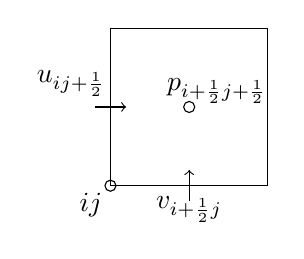
\begin{tikzpicture}
\draw (0,0) rectangle (2,2);
\draw (1.35,1.2) node {$p_{i+\frac{1}{2}j+\frac{1}{2}}$};
\draw[->] (1,-0.2) -- (1,0.2);
\draw (1,-0.3) node {$v_{i+\frac{1}{2}j}$};
\draw[->] (-0.2,1) -- (0.2,1);
\draw (-0.5,1.3) node {$u_{ij+\frac{1}{2}}$};
\draw (1,1) circle (2pt);

\draw (0,0) circle (2pt);
\draw (-0.25,-0.25) node {$ij$};
\end{tikzpicture}
\caption{Cell of the staggered grid\label{grid-cell}}
\end{figure}

\begin{figure}[!ht]
\centering
\tikzstyle{help lines}+=[dashed]
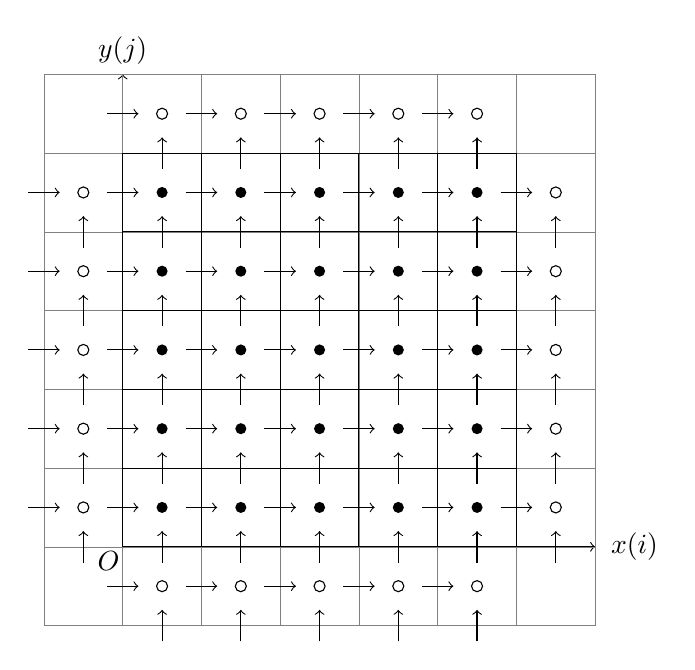
\begin{tikzpicture}
%axes
\draw[->] (0,5) -- (xyz cs:y=6);
\draw (0,6.3) node {$y(j)$};
\draw[->] (5,0) -- (xyz cs:x=6);
\draw (6.5,0) node {$x(i)$};
\draw (-0.18,-0.18) node {$O$};
%grid
\draw[style=help lines] (-1,-1) grid +(7,7);
\draw (0,0) grid +(5,5);
%internal p points
\foreach \x in {0.5,1.5,2.5,3.5,4.5}
  \foreach \y in {0.5,1.5,2.5,3.5,4.5}
  {
  \fill (canvas cs:x=\x cm,y=\y cm) circle (2pt);
}
%External p points
\foreach \x in {0.5,1.5,2.5,3.5,4.5}
  \draw (\x,-0.5) circle (2pt);
\foreach \y in {0.5,1.5,2.5,3.5,4.5}
  \draw (5.5,\y) circle (2pt);
\foreach \y in {0.5,1.5,2.5,3.5,4.5}
  \draw (-0.5,\y) circle (2pt);
\foreach \x in {0.5,1.5,2.5,3.5,4.5}
  \draw (\x,5.5) circle (2pt);
%Internal Horizontal Velocities Points
\foreach \x in {-1.2,-0.2,0.8,1.8,2.8,3.8,4.8}
  \foreach \y in {0.5,1.5,2.5,3.5,4.5}
  {
  \draw[->] (\x,\y) -- (\x+0.4,\y);
}
%External Horizontal Velocities Points
\foreach \x in {-.2,0.8,1.8,2.8,3.8}
  \draw[->] (\x,5.5) -- (\x+0.4,5.5);
\foreach \x in {-.2,0.8,1.8,2.8,3.8}
  \draw[->] (\x,-.5) -- (\x+0.4,-.5);
%Internal Vertical Velocities Points
\foreach \x in {0.5,1.5,2.5,3.5,4.5}
  \foreach \y in {-1.2,-0.2,0.8,1.8,2.8,3.8,4.8}
  {
  \draw[->] (\x,\y) -- (\x,\y+0.4);
}
%External Vertical Velocities Points
\foreach \y in {-0.2,0.8,1.8,2.8,3.8}
  \draw[->] (5.5,\y) -- (5.5,\y+0.4);
\foreach \y in {-0.2,0.8,1.8,2.8,3.8}
  \draw[->] (-.5,\y) -- (-.5,\y+0.4);
\end{tikzpicture}
\caption{Staggered-grid. Dark circles are internal points, while empty ones are part of the extra layer\label{staggered-grid}}
\end{figure}

The code for the simulator was made with aid of programming language Julia, more information about this language is available at \cite{JuliaProgramming}. Julia offers several linear algebra packages that are easy to use and very efficient. Graphics were made using Python's graphical packages \cite{matplotlib}. Codes and articles of this project are hosted on GitHub\footnote{https://github.com/ataias/ferrofluidos}. %In the Julia language, matrices are indexed from 1 to $n$. This is different from C, because its indexing starts from 0.

\section{Governing Equations}
\subsection{Hidrodynamics}
Equations \ref{navierstokes} and \ref{navierincompressibilidade} govern the flow of an incompressible fluid. The first one is the Navier-Stokes equation \cite{batchelor}, while the second one is the condition for incompressibility:

\begin{eqnarray}
\left( \frac{\partial {\textbf{v}}}{\partial t}+\textbf{v}\cdot\nabla \textbf{v} \right)=-\nabla p+\frac{1}{\mathit{Re}}\nabla^2 \textbf{v} + \textbf{f}\label{navierstokes},\\
\nabla\cdot\textbf{v}=0.\label{navierincompressibilidade}
\end{eqnarray}

In the latter equations, some terms are presented: $\mathbf{v}$ is the velocity, $p$ stands for pressure and $\mathbf{f}$ is the force acting on the fluid, which is, in our case, created by a magnetic field. The Reynolds number $\mathit{Re}$ is given by 

\begin{eqnarray}
\mathit{Re}=\frac{\rho L U}{\mu},
\end{eqnarray}

in which $\rho$ is the density of the fluid, $L$ is a characteristic linear dimension, $U$ is maximum speed in the cavity and $\mu$ is the dynamic viscosity.

Computer solutions require certain conditions on the time step and spacing of grid points. As well described on \cite{hinchLectureNotes}, the requirements are: stable diffusion, 
\begin{equation}
\Delta t < \frac{1}{4}\mathit{Re}\Delta x^2, \label{stablediffusion}
\end{equation} 

stable advection, the CFL condition,
\begin{equation}
\Delta t < \frac{\Delta x}{U}, \label{stableadvection}
\end{equation}

 and to resolve well the hydrodynamic boundary layer,  
 \begin{eqnarray}
\Delta x &<& \frac{1}{\mathit{Re}}. \label{boundarylayer}
\end{eqnarray} 

If the time-stepping conditions are not satisfied, the routine will try to solve the flow faster than the laws of physics allow. The result is an incorrect solution or divergency of the solution.


The Navier-Stokes equation is thorough, encompassing several types of flow. A specific solution is found by stating its boundary conditions. For the current work, the conditions are

\begin{eqnarray}
u(x,1) & = & \sin^2(\pi x),\\
u(x,0) & = & u(0,y) = u(1,y) = 0,\\
v(x,0) & = & v(x,1) = v(0, y) = v(1, y) = 0.
\end{eqnarray}

\subsection{Magnetism}
Besides the hydrodynamics equations and conditions, the magnetic force  in Equation 1, $\mathbf{f}$, must be computed. From Maxwell's theory, Equation \ref{secondmagneticequation} is obtained:

\begin{eqnarray}
\nabla\cdot \mathbf{B} & = & 0\label{secondmagneticequation}.
\end{eqnarray}

and, from a magnetizable medium, we have Equation \ref{firstmagneticequation}:

\begin{eqnarray}
\mathbf{B} &=& \mu_0(\mathbf{M}+\mathbf{H}).\label{firstmagneticequation}
\end{eqnarray}

From the latter equations, it is possible to conclude that 

\begin{eqnarray}
\nabla\cdot\mathbf{H} = -\nabla\cdot \mathbf{M}\label{mh1}.
\end{eqnarray}

The magnetostatic regime of the Maxwell's equations implies \begin{equation}\nabla\times \mathbf{H} = \mathbf{0},
\end{equation} 

which indicates there is a potential field $\phi$ that satisfies \begin{equation}\mathbf{H} = -\nabla \phi.\label{Hphipotencial}\end{equation} With these last equations, it is possible to obtain \begin{eqnarray}
\nabla^2\phi &=& \nabla\cdot \mathbf{M}.\label{eqcampomag}
\end{eqnarray}

This is a Poisson equation that will give $\phi$ according the the local magnetization of the ferrofluid. The superparamagnetic case is being considered, what implies 
\begin{equation}\mathbf{M} = \chi \mathbf{H}.\end{equation}


Nevertheless, the potential $\phi$ cannot be introduced directly in the Navier-Stokes equation. What is needed is a relation that gives the magnetic force, which could then be incorporated in the fluid equations. The magnetic force is \begin{equation}
	\mathbf{f} = \mathrm{C}_{\mathrm{pm}}\; \mathbf{M}\cdot \nabla \mathbf{H},\label{magneticforce}\end{equation} in which $\mathrm{C}_{\mathrm{pm}}$ is the magnetic Reynolds number, given by 
\begin{eqnarray}
\mathrm{C}_{\mathrm{pm}} & = & \frac{\mu_0 H_0^2}{\rho u^2}.\label{cpm}
\end{eqnarray}

The boundary conditions were not yet determined for the potential field $\phi$. To derive those conditions, an applied magnetic field $\mathbf{H}$ was considered and the continuity requirement was imposed for the normal component of $\mathbf{B}$, Equation \ref{firstmagneticequation}. This continuity can be mathematically represented by \begin{equation}\left(\mathbf{B}_{\mathrm{out}} - \mathbf{B}_{\mathrm{in}}\right)\cdot \mathbf{n} = 0 \label{normalconditionB}.\end{equation} 

From this, Equation \ref{normalConditionB2} can be obtained:

\begin{eqnarray}
\mu_0 (H_{\mathrm{out}}^{\mathrm{n}} + M_{\mathrm{out}}^{\mathrm{n}}) &=&  \mu_0(H_{\mathrm{in}}^{\mathrm{n}}+M_{\mathrm{in}}^{\mathrm{n}}).\label{normalConditionB2}
\end{eqnarray}

The medium outside is air and therefore its magnetization $M_{\mathrm{out}}^{\mathrm{n}}$ is zero. The term $H_{\mathrm{out}}^{\mathrm{n}}$ is substituted following  Equation \ref{Hphipotencial}, resulting  in Equation \ref{nablaphid}:

\begin{eqnarray}
\nabla\phi_{\mathrm{d}}^{\mathrm{n}} & = & -H_{\mathrm{f}}^{\mathrm{n}} + M_{\mathrm{d}}^{\mathrm{n}}. \label{nablaphid}
\end{eqnarray}

From that, Neumann boundary conditions can be obtained for Equation \ref{eqcampomag}. For the sake of clarity, they are presented in Equations \ref{condition1phi} to \ref{condition4phi}. The subscripts are indicating matrix indices.

\begin{eqnarray}
\left.\frac{\partial \phi}{\partial x}\right|_{\mathrm{left}}\;\;&\approx&- H^{x}_{2,j} + M^{x}_{2,j}\label{condition1phi}\\
\left.\frac{\partial \phi}{\partial x}\right|_{\mathrm{right}}&\approx&- H^{x}_{n,j} + M^{x}_{n,j}\\
\left.\frac{\partial \phi}{\partial y}\right|_{\mathrm{lower}}&\approx&- H^{y}_{i,2} + M^{y}_{i,2}\\
\left.\frac{\partial \phi}{\partial y}\right|_{\mathrm{upper}}&\approx&- H^{y}_{i,n} + M^{y}_{i,n}\label{condition4phi}
\end{eqnarray}

\section{Solution Method}
\subsection{Time-splitting}
In order to discretize the Navier-Stokes equation, an expansion is performed in directions $x$ and $y$ to obtain scalar equations and then finite differences of second order are applied. Nevertheless, a naive application of the discretized formulas will not yield a proper solution, as the fluid flow equation is highly non-linear due to its convective term $\mathbf{v}\cdot \nabla \mathbf{v}$. Also, pressure is not known in advance so, while it is needed at each time step, it is also an unknown that must be found. A method developed by Chorin, named time-splitting, and described in \cite{Chorin1997118} was used to resolve this problem. Firstly, one starts by applying finite differences for the velocity derivative with respect to time and then manipulating by summing and subtracting $\mathbf{v}^*$ in the numerator, as in

\begin{equation}
\frac{\partial \textbf{v}}{\partial t}\approx \frac{\textbf{v}^{n+1}-\textbf{v}^n}{\Delta t}=\frac{\textbf{v}^{n+1}-\textbf{v}^*}{\Delta t}+\frac{\textbf{v}^{*}-\textbf{v}^n}{\Delta t}, \label{vdottimesplitting}
\end{equation}

in which $\mathbf{v}^n$ is the velocity at the current time-step and $\mathbf{v}^{n+1}$ is the velocity one time-step in the future.

The aforementioned technique imposes on the term $\frac{\textbf{v}^{n+1}-\textbf{v}^*}{\Delta t}$ of Equation \ref{vdottimesplitting} a sufficiency to solve the pressure field: 
\begin{equation}\frac{\textbf{v}^{n+1}-\textbf{v}^*}{\Delta t}=-\frac{1}{\rho}\nabla p\label{equacaoprepressao}.\end{equation}

 Notice that Equation \ref{equacaoprepressao} already shows a relation between $\mathbf{v}^{n+1}$ and $\mathbf{v}^{*}$, a correlation that is pertinent because it is used to obtain the velocity in the next time step after pressure is calculated.


The other term, $\frac{\textbf{v}^{*}-\textbf{v}^n}{\Delta t}$, is responsible for all the terms of Equation \ref{navierstokes}, except the pressure gradient term that is already considered on Equation \ref{equacaoprepressao}: \begin{eqnarray}
\frac{\textbf{v}^{*}-\textbf{v}^n}{\Delta t}&=& \nu\nabla ^2 \textbf{v} + \frac{\textbf{f}}{\rho} - \textbf{v}\cdot \nabla \textbf{v}\label{equacaovestrela}
\end{eqnarray}

The term $\mathbf{v}^*$ can be isolated in Equation \ref{equacaovestrela} and then calculated easily as only known terms from time step $n$ are involved in the aforementioned equation.

As a means to calculate $p$, the divergence operator is applied to both sides of Equation \ref{equacaoprepressao}: \begin{eqnarray}
	-\frac{1}{\rho}\nabla\cdot\nabla p & = &\nabla\cdot \left(\frac{\textbf{v}^{n+1}-\textbf{v}^*}{\Delta t}\right).
\end{eqnarray}

As $\mathbf{v}^{n+1}$ has to obbey the incompressibility condition, its divergence is zero, with the remaining equation being transformed into a Poisson equation: \begin{eqnarray}
\nabla^2 p & = & \frac{\rho}{\Delta t}\nabla\cdot \textbf{v}^{*}.	 \label{pressureVStar}
\end{eqnarray}



Now that Equation \ref{pressureVStar} is available, it is easier to devise a solution to the problem, as only $\mathbf{v}^*$ is needed and it is already a known value because of Equation \ref{equacaovestrela}. However, nothing was stated about the boundary conditions this problem involves. For that, it is better to expand the Navier-Stokes equation, as in Equations \ref{navierX} and \ref{navierY}.

\begin{eqnarray}
\frac{\partial u}{\partial t}+u\frac{\partial u}{\partial x}+v\frac{\partial
u}{\partial y}=-\frac{1}{\rho}\frac{\partial p}{\partial
x}+\nu\left(\frac{\partial^2 u}{\partial^2 x}+\frac{\partial^2 u}{\partial^2
y}\right)+f_x \label{navierX}\\
\frac{\partial v}{\partial t}+u\frac{\partial v}{\partial x}+v\frac{\partial
v}{\partial y}=-\frac{1}{\rho}\frac{\partial p}{\partial
y}+\nu\left(\frac{\partial^2 v}{\partial^2 x}+\frac{\partial^2 v}{\partial^2
y}\right)+f_y \label{navierY}
\end{eqnarray}

Given the two latter equations, boundary conditions on the walls can be applied. Many terms are zero on the wall, and the result is presented in Equations \ref{paredesVerticais} and \ref{paredesHorizontais}. Notice that those are Neumann boundary conditions.

\begin{eqnarray}
\frac{\partial p}{\partial x}\Bigg|_{\textrm{wall}}&=&\rho\nu\frac{\partial^2
u}{\partial x^2}\Bigg|_{\textrm{wall}}+\rho f_x\label{paredesVerticais}\\
\frac{\partial p}{\partial y}\Bigg|_{\textrm{wall}}&=&\rho\nu\frac{\partial^2
v}{\partial y^2}\Bigg|_{\textrm{wall}}+\rho f_y\label{paredesHorizontais}
\end{eqnarray}

As the four walls have flux conditions, there are infinitely many solutions that differ only by a constant. A point in the mesh can be specified arbitrarily so that the program converges to a specific solution. This is allowed in our problem, as pressure itself is not directly needed, but only its gradient.

There is one last step to obtain $\mathbf{v}^{n+1}$, but this is quite straightforward: Equation \ref{nextStepV} must be computed. It is an explicit equation with known terms at this stage.

\begin{eqnarray}
	\mathbf{v}^{n+1} & = & \mathbf{v}^*  - \frac{\Delta t}{\rho} \nabla p \label{nextStepV}
\end{eqnarray}

The three time-splitting steps were presented, but not all their discretizations. The discretization for step 1 is on Equations \ref{step1-3} and \ref{step1-4}. Equations \ref{step1-1} and \ref{step1-2} are variables made do ease the understanding of the main equations for this step. Equation \ref{step1-1} is the sum of cell points around $ij$, while \ref{step1-2} is a linear interpolation to obtain $u$ and $v$ at desired points that are not available directly in the staggered grid.  For each inner point of the mesh, the equations presented are applied in an explicit form.

\begin{eqnarray}
\textbf{v}_{ij}^s&=&(\SumFour{u})\textbf{i} \nonumber \\&+& (\SumFour{v})\textbf{j} \label{step1-1}\\
\textbf{v}_{ij}^t&=&0.25(u_{ij}^n+u_{i+1j}^n+u_{i+1j-1}^n+u_{ij-1}^n)\textbf{i} \nonumber \\ &+& 0.25(v_{ij}^n+v_{i-1j}^n+v_{i-1j+1}^n+v_{ij+1}^n)\textbf{j} \label{step1-2}
\end{eqnarray}
%------------------- u* -------------------
\begin{eqnarray}
u_{ij}^{*}&=&u_{ij}^n+\frac{\Delta t}{\rho}\left[\mu\left(\frac{u_{ij}^s-4u_{ij}^n}{\Delta
x^2}\right)+Fx_{ij}^n\right] + \nonumber \\
&-&\left[u_{ij}^n(u_{i+1j}^n-u_{i-1j}^n)+ \right.\nonumber \\
&+& \left. v_{ij}^t(u_{ij+1}^n-u_{ij-1}^n)\right]\frac{\Delta t}{2\Delta x}\label{step1-3}
\end{eqnarray}
%------------------- v* ------------------
\begin{eqnarray}
v_{ij}^{*}&=&v_{ij}+\frac{\Delta t}{\rho}\left[\mu\left(\frac{v_{ij}^s-4v_{ij}^n}{\Delta
x^2}\right)+Fy_{ij}^n\right] \nonumber \\
&-&\left[u_{ij}^t (v_{i+1j}^n-v_{i-1j}^n)+ \right.\nonumber \\
&+& \left. v_{ij}^n(v_{ij+1}^n-v_{ij-1}^n)\right]\frac{\Delta t}{2\Delta x}\label{step1-4}
\end{eqnarray}

\subsection{Poisson equations}

The second step, solving for the pressure, can have an explicit or implicit solution method. Both methods were used, and the implicit one is much faster, so it is presented here. The hardest part of this method is that one can not apply the discretized equations directly, but it is necessary to form a linear system from it. For the implicit method, matrix $A$ and vector $b$ are needed to solve system $Ax = b$. The pressure elements are in the unknown $x$. This system gets very large, but most of the elements in matrix $A$ are 0, so $A$ is a sparse matrix. Firstly, let's present the steps to obtain $A$ and $b$:

\begin{figure}[!ht]
\centering
\tikzstyle{help lines}+=[dashed]% 
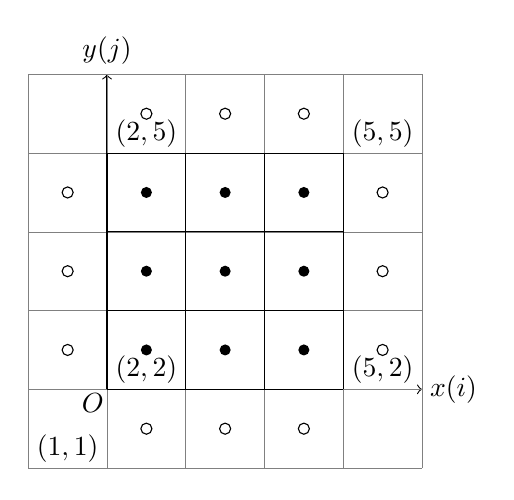
\begin{tikzpicture}
%axes
\draw[->] (0,3) -- (xyz cs:y=4);
\draw (0,4.3) node {$y(j)$};
\draw[->] (3,0) -- (xyz cs:x=4);
\draw (4.4,0) node {$x(i)$};
\draw (-0.18,-0.18) node {$O$};
\draw (-0.5,-0.75) node {$(1,1)$};
\draw (0.5,0.25) node {$(2,2)$};
\draw (3.5,3.25) node {$(5,5)$};
\draw (0.5,3.25) node {$(2,5)$};
\draw (3.5,0.25) node {$(5,2)$};

%grid
\draw[style=help lines] (-1,-1) grid +(5,5);
\draw (0,0) grid +(3,3);
%internal p points
\foreach \x in {0.5,1.5,2.5}
  \foreach \y in {0.5,1.5,2.5}
  {
  \fill (canvas cs:x=\x cm,y=\y cm) circle (2pt);
}
%External p points
\foreach \x in {0.5,1.5,2.5}
  \draw (\x,-0.5) circle (2pt);
\foreach \y in {0.5,1.5,2.5}
  \draw (3.5,\y) circle (2pt);
\foreach \y in {0.5,1.5,2.5}
  \draw (-0.5,\y) circle (2pt);
\foreach \x in {0.5,1.5,2.5}
  \draw (\x,3.5) circle (2pt);

\end{tikzpicture} 
\caption{Example grid to solve for pressure\label{examplePressureGrid}}
\end{figure}

Consider a $5\times 5$ grid as in Figure \ref{examplePressureGrid}. The equation to be solved is Equation \ref{poissonEquation}, a generic poisson equation. 
\begin{equation}
\nabla^2 p = \frac{\partial^2 p}{\partial x^2} + \frac{\partial^2 p}{\partial y^2} = g(x,y)\label{poissonEquation}
\end{equation}

Using second order central differences, Equation \ref{poissonSecond} is obtained. This equation is valid for internal points (black points in Figure \ref{examplePressureGrid}).

\begin{eqnarray}
\frac{p_{i-1j} - 2p_{ij} + p_{i+1j}}{\Delta x^2}	+ \frac{p_{ij-1} - 2p_{ij} + p_{ij+1}}{\Delta x^2} = g_{ij}\label{poissonSecond}
\end{eqnarray}

If term $p_{ij}$ is isolated in Equation \ref{poissonSecond}, an explicit equation is obtained to all the internal points. The external points will be obtained from boundary conditions. Nevertheless, what is needed is an implicit representation of the system. For that, all the equations need to be considered and then organized in matrix form. The first equations for the internal points are presented in Equations \ref{internalPoissonEq1} to \ref{internalPoissonEq3}. Equations for the other internal points (more 6 equations) are easily obtainable.

\begin{eqnarray}
-4p_{22} + p_{32} + \boldsymbol{p_{12}} + p_{23} + \boldsymbol{p_{21}} &=& \Delta x^2 g_{22} \label{internalPoissonEq1}\\
-4p_{23} + p_{33} + \boldsymbol{p_{13}} + p_{24} + p_{22} &=& \Delta x^2 g_{23}\label{internalPoissonEq2}\\
-4p_{24} + p_{34} + \boldsymbol{p_{14}} + \boldsymbol{p_{25}} + p_{23} &=& \Delta x^2 g_{24}\label{internalPoissonEq3}
\end{eqnarray}

The pressure points written in bold letters are boundary points. This means there exists an equation that can account for them. There are twelve external points and from the boundary conditions it is easy to get the twelve equations. Equations \ref{pressureBoundary1} to \ref{pressureBoundary4} can have its indices substituted in order to get 12 equations.

\begin{eqnarray}
\frac{\partial p}{\partial x}\left(0, y\right) &=& p_x\left(0, y\right)  \approx  (p_{2j} - p_{1j})/\Delta x \label{pressureBoundary1}\\
\frac{\partial p}{\partial x}\left(1, y\right) &=& p_x\left(1, y\right)  \approx  (u_{5j} - u_{4j})/\Delta x\\
\frac{\partial p}{\partial y}\left(x, 0\right) &=& p_y\left(x, 0\right)  \approx (p_{i2} - p_{i1})/\Delta x\\
\frac{\partial p}{\partial y}\left(x, 0\right) &=& u_y\left(x, 0\right)  \approx  (p_{i5} - p_{i4})/\Delta x\label{pressureBoundary4}
\end{eqnarray}

From the 21 equations obtained, a rearrangement can be done to obtain matrix $A$, which is presented in Equation \ref{matrixAnulleigen}. The $b$ vector is in Equation \ref{bPartnulleigen}. Nevertheless, one of the Eigenvalues of this system is zero, so the matrix is not invertible. This problem has to do with the fact that there are only Neumann boundary conditions and many differing-by-constant solutions are possible. To solve this problem, one value of the mesh must be imposed and the cell to be chosen can be any but one of the corner points, as they don't take any part on the equations. 

\begin{equation}
\resizebox{.95\hsize}{!}{$
\left[\begin{array}{ccccccccc}
-2 & 1 & 0 & 1 & 0 & 0 & 0 & 0 & 0\\
1 & -3 & 1 & 0 & 1 & 0 & 0 & 0 & 0\\
0 & 1 & -2 & 0 & 0 & 1 & 0 & 0 & 0\\
1 & 0 & 0 & -3 & 1 & 0 & 1 & 0 & 0\\
0 & 1 & 0 & 1 & -4 & 1 & 0 & 1 & 0\\
0 & 0 & 1 & 0 & 1 & -3 & 0 & 0 & 1\\
0 & 0 & 0 & 1 & 0 & 0 & -2 & 1 & 0\\
0 & 0 & 0 & 0 & 1 & 0 & 1 & -3 & 1\\
0 & 0 & 0 & 0 & 0 & 1 & 0 & 1 & -2 
\end{array}\right] \left[\begin{array}{c}
p_{22}\\ p_{23}\\ p_{24}	\\ p_{32}\\ p_{33}\\ p_{34}\\ p_{42}\\p_{43} \\u_{44}
\end{array}\right] = b$} \label{matrixAnulleigen}
\end{equation}

\begin{eqnarray}
b & = & \Delta x\left[\begin{array}{c}
p_x\left(0, \frac{\Delta x}{2}\right) + p_y\left(\frac{\Delta x}{2},0\right)\\
u_x\left(0, \frac{3\Delta x}{2}\right)\\
p_x\left(0, \frac{5\Delta x}{2}\right) - p_y\left(\frac{\Delta x}{2},1\right)\\
p_y\left(\frac{3\Delta x}{2},0\right)\\
0 \\
-p_y\left(\frac{3\Delta x}{2},1\right)\\
-p_x\left(1, \frac{\Delta x}{2}\right) + p_y\left(\frac{5\Delta x}{2},0\right)\\
-u_x\left(1, \frac{3\Delta x}{2}\right)\\
-p_x\left(1, \frac{5\Delta x}{2}\right) - p_y\left(\frac{5\Delta x}{2}, 1\right)
\end{array}\right] \nonumber\\
&+& \Delta x^2 \left[
g_{22}\; g_{23}\; g_{24}\; g_{32}\; g_{33}\; g_{34}\; g_{42}\; g_{43} \; g_{44}
\right]^T \label{bPartnulleigen}
\end{eqnarray}

For our problem, $p_{12} = 0$ was chosen. This updates one element of the matrix and one element of the vector. The updated values are shown in Equations \ref{aupdate} and \ref{bupdate}.

\begin{eqnarray}
A[1,1] &=& -3 \label{aupdate} \\
b[1] & = & p_y\left(\frac{\Delta x}{2},0\right)\Delta x + \Delta x^2 g_{22} \label{bupdate}
\end{eqnarray}

The equations just presented can be coded to define matrix $A$ and vector $b$, but to actually obtain the vector $x$ of pressure points the system must be solved. A sparse matrix solver available in Julia\footnote{http://julialang.org} is used. It uses a Cholesky factorization in order to solve the system. As the matrix is fixed, the factorization can be done once and for every other time-step the fatorized matrix is used. This is a performance-wise decision.

For the magnetism parts, it was only necessary to use finite differences on the governing equations. The Poisson implicit elements obtained in this section are also used for the magnetic part. The rest are explicit applications of the finite differences equations obtained.



\section{Results}

It is important to validate the code. As part of the solution method, tests of the Poisson routine and of the discretization of the Navier-Stokes equation are made. The Poisson test is to check the error when comparing a computed result with the actual analytical function that solves the PDE. The second test applies to the Navier-Stokes equation and also for the Poisson one: verifying how the error decays according to an increase in mesh size. As all the discrete formulas used are of second order, this error should decay quadratically. The ``Results'' section will present both of these tests. Also, Navier-Stokes with magnetism will be tested to check the order of the discretization.


\subsection{Validation of the Poisson Solver}

The implementation of the solver was evaluated by testing a few different problems, but only a succinct presentation is done here with one problem: Equation \ref{poissonTest1}. 

\begin{eqnarray}
\left\{\begin{array}{ccl}
\nabla^2u(x,y) & = & 0,\\
u_x(1,y) & = & \cos 2\pi y,\\
u_n(x,y) & = & 0, \textrm{otherwise, on the boundary}.
\end{array}\right. \label{poissonTest1}
\end{eqnarray}

Its analytical solution is:

\begin{eqnarray}
u(x,y) & = & \frac{\cosh 2\pi x}{2\pi \sinh 2\pi}\cos 2 \pi y .\label{solutionPoissonTest1}
\end{eqnarray}


The Poisson validation routine returns the middle point difference on the grid that was found, this value is then divided by the real value on that point and multiplied by 100 to get a percentage. The maximum grid size used was $320\times 320$. This one had an error smaller than $0.05\%$. The results for different grid sizes are presented in Figure \ref{errorPoissonTest}. It is easy to see that the error decays quadratically, what was expected due to the second order finite differences that were used.



\begin{eqnarray}
u(x,y) & = & \frac{\cosh 2\pi x}{2\pi \sinh 2\pi}\cos 2 \pi y \label{solutionPoissonTest1}
\end{eqnarray}

\begin{figure}[!ht]
\centering
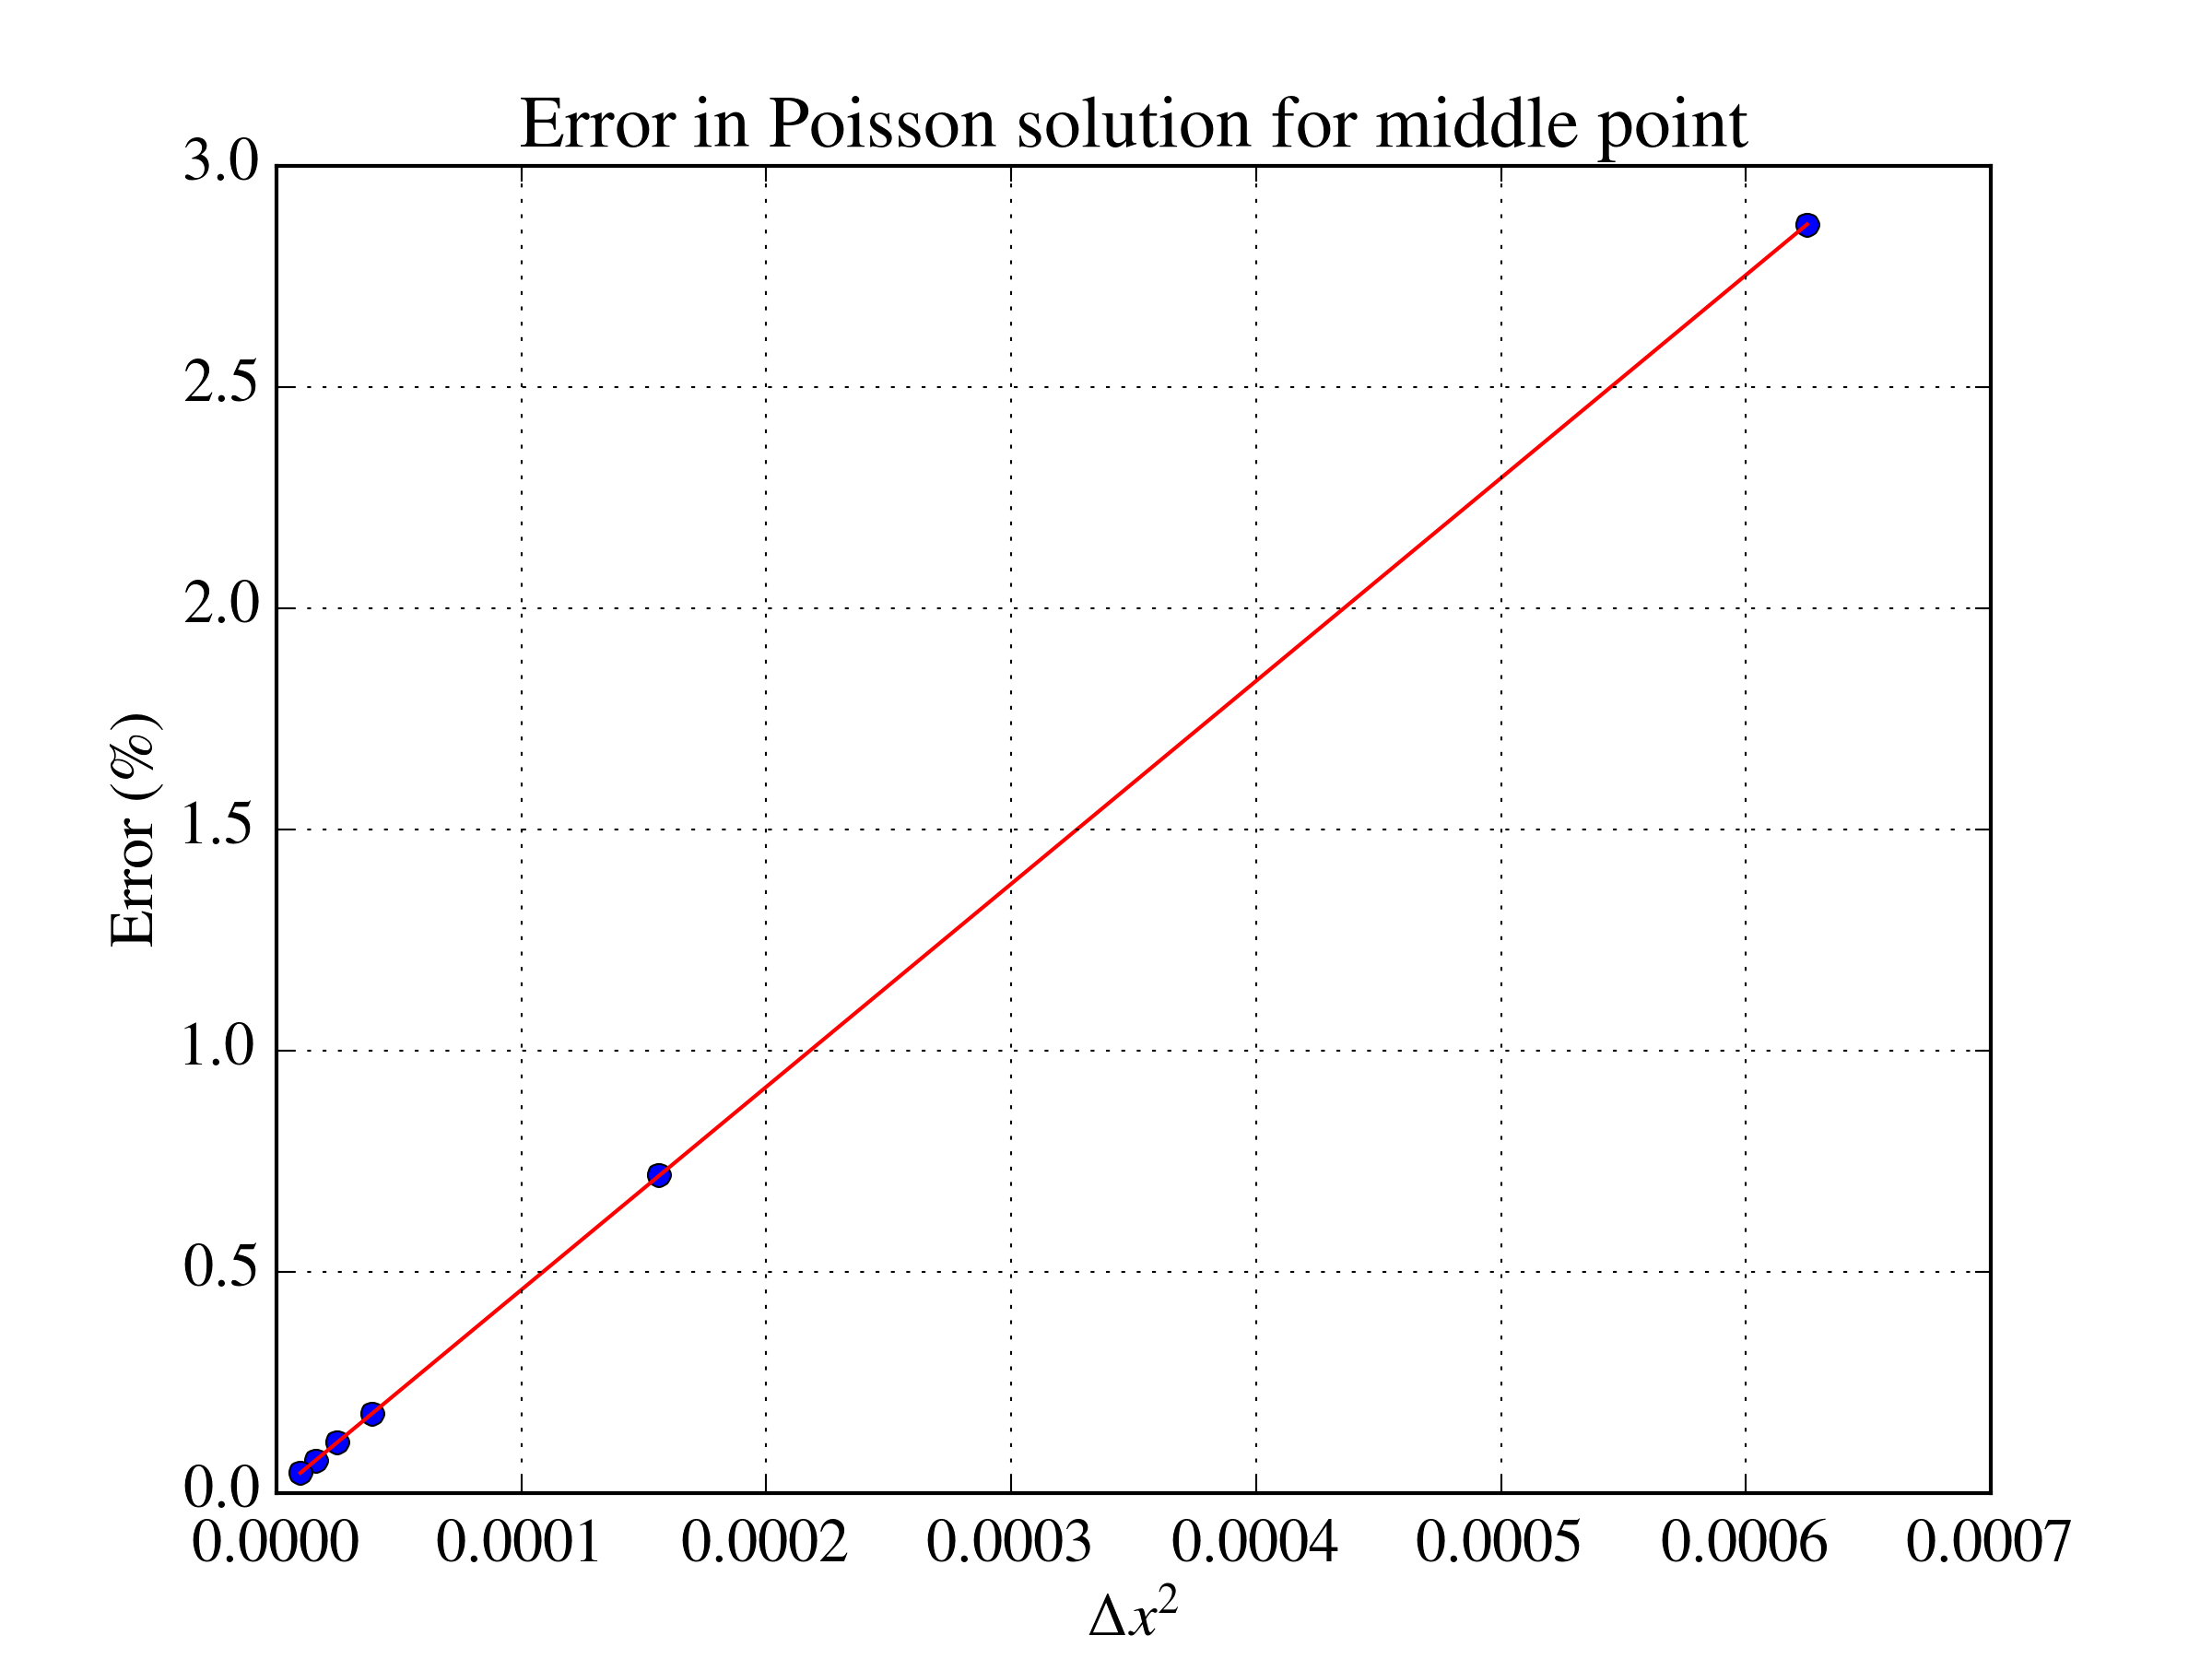
\includegraphics[width=\linewidth]{figures/validatePoissonP2}
\caption{Error evolving according to grid size. Higher grid sizes are closer to left-bottom corner. Error decays quadratically. Comparison with analytical solution. Grid sizes from $40\times 40$ to $320\times 320$. \label{errorPoissonTest}}
\end{figure}

\subsection{Validation of the Navier-Stokes routine}

Validation for the hydrodynamics is presented on Figure \ref{hydrodynamicsTest}. Reynolds is chosen to be 40. The error will be compared against the solution of grid size $200\times 200$, as access to the analytical solution is not possible. The important point to evaluate is that the error decays quadratically, what can be assessed from the image for simplicity. Vorticity was used instead of velocity because it is a scalar that accounts for both velocity terms. Note that the error corresponds to the base case of $200\times 200$.

\begin{figure}[!t]
\centering
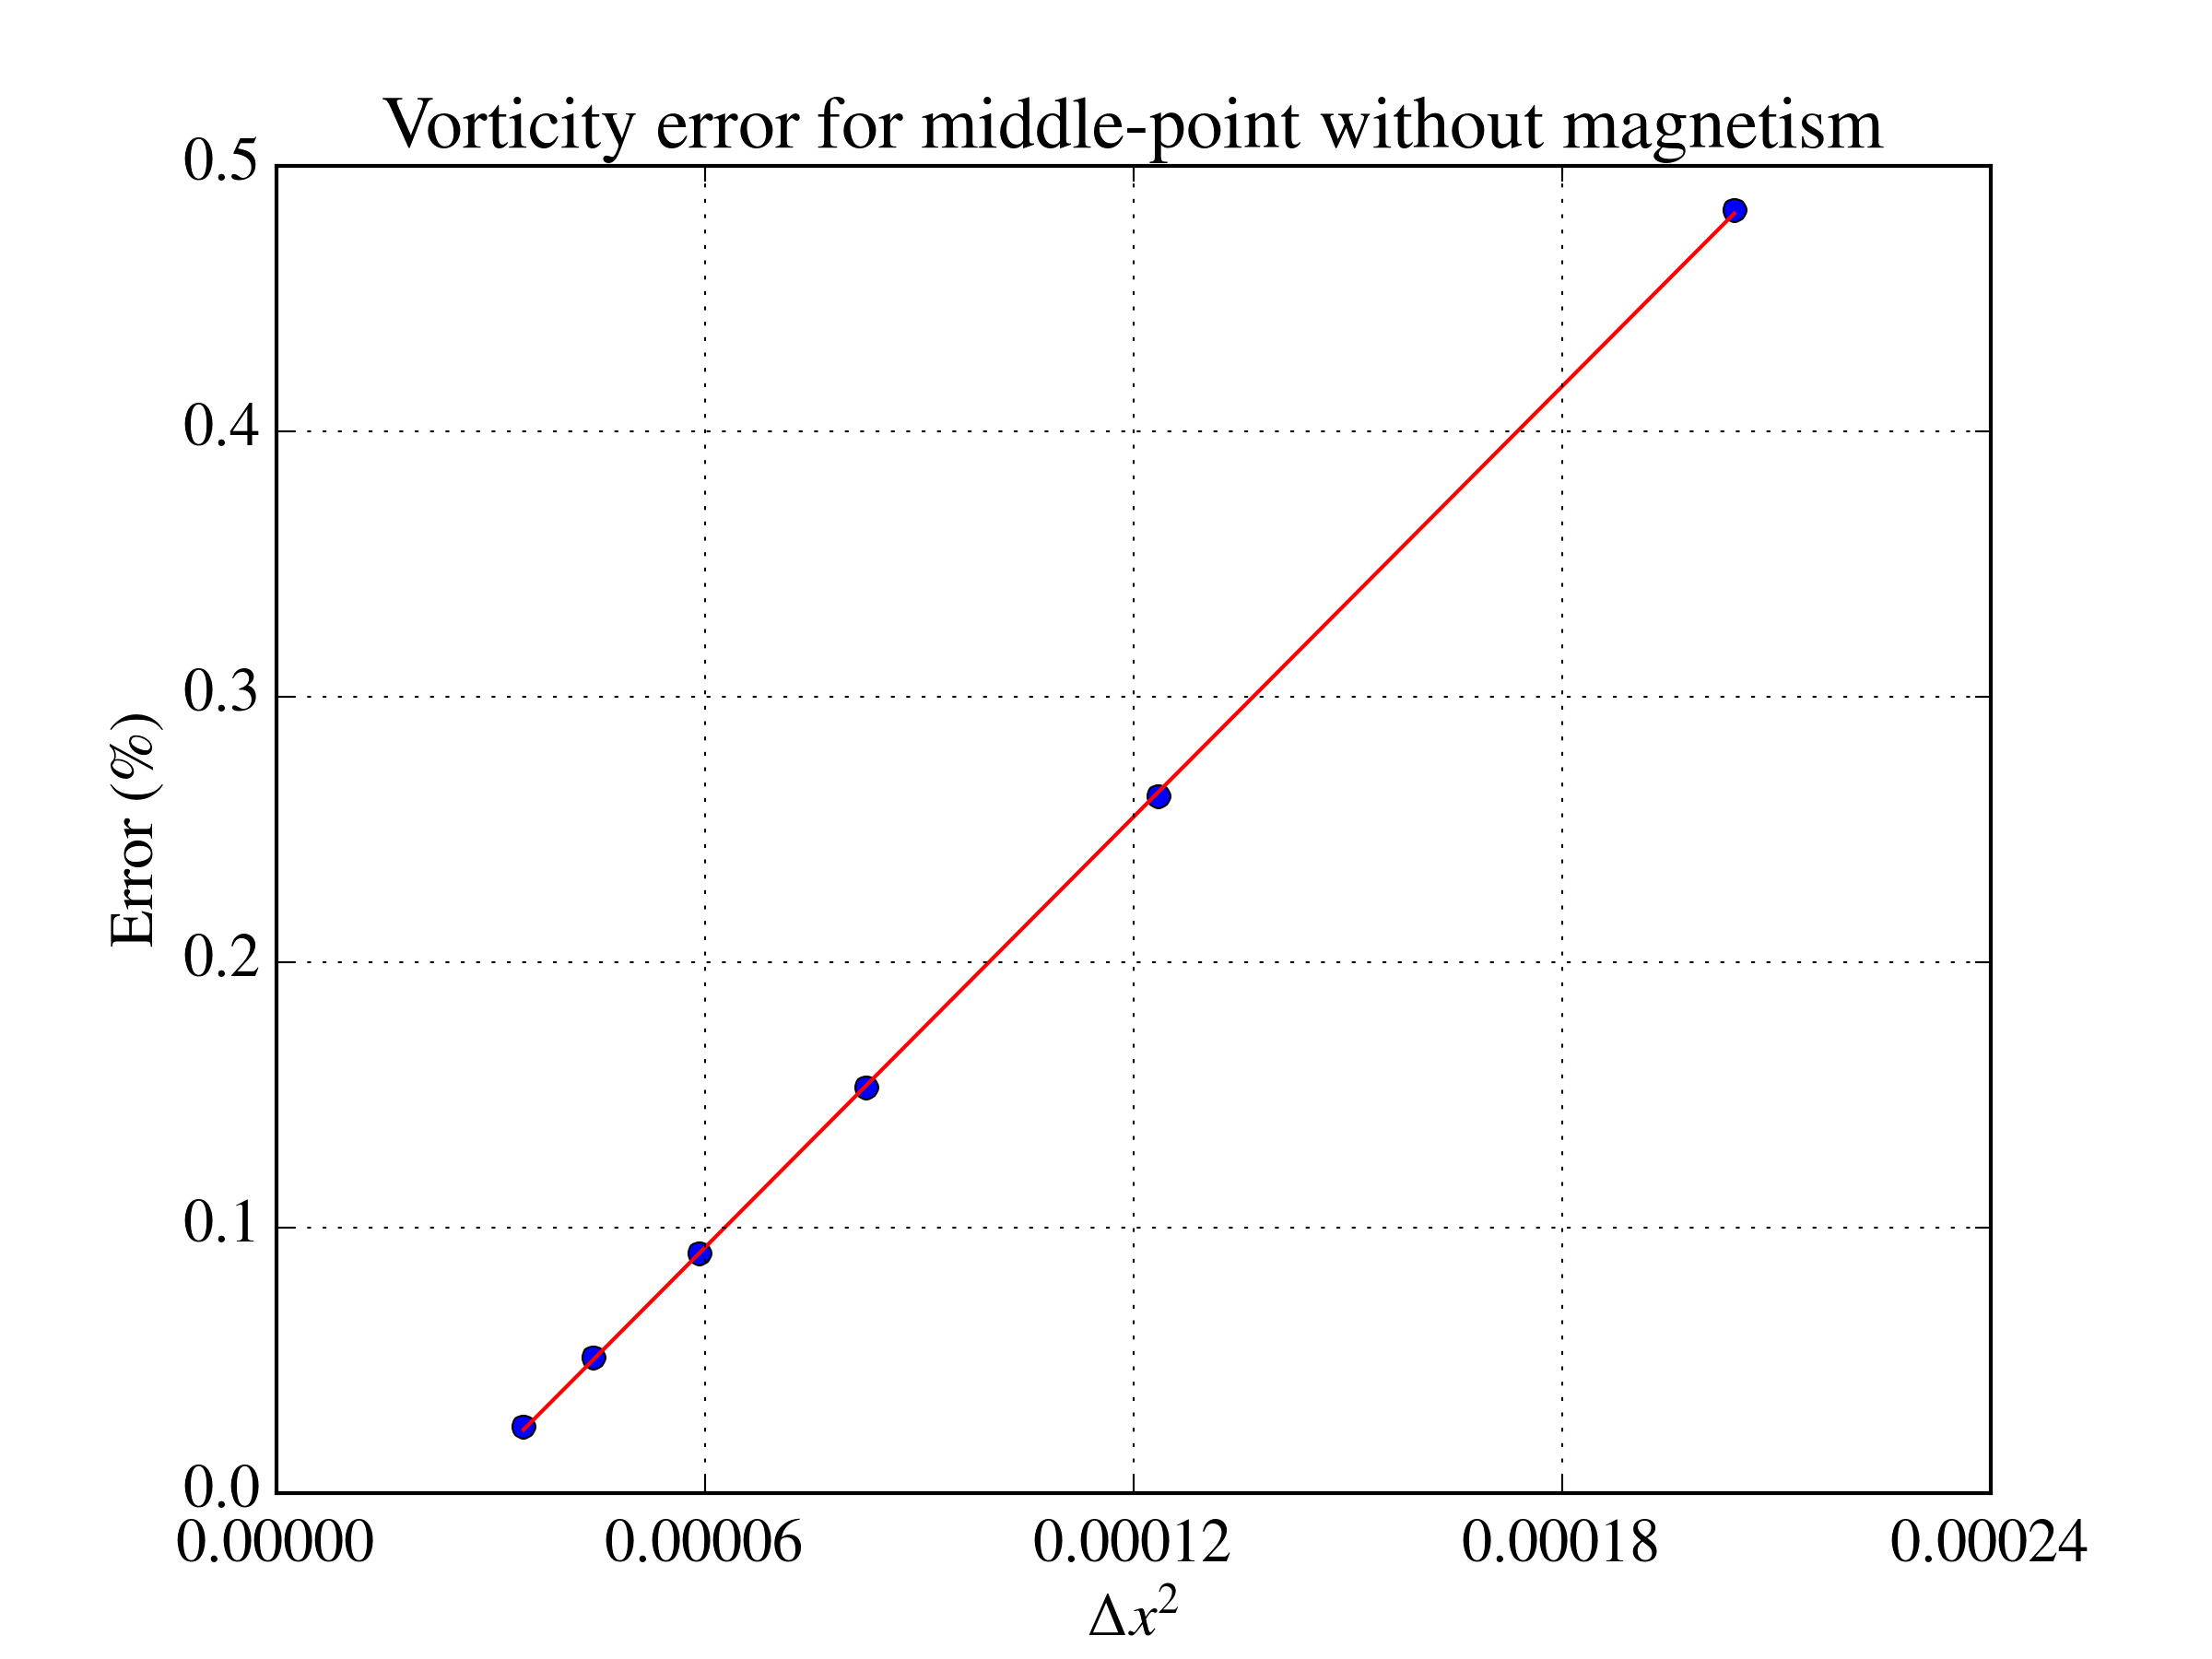
\includegraphics[width=\linewidth]{figures/validateHydrodynamicsRe40}
\caption{Error evolving according to grid size. Higher grid sizes are closer to left-bottom corner. Error decays quadratically. Comparison with solution of $200\times 200$ grid. Grid sizes from $70\times 70$ to $170\times 170$. \label{hydrodynamicsTest}}
\end{figure}

A similar test was used when magnetism is present. This case has a force $\mathbf{f}$ that differs from zero. Magnetic parameters chosen are $\chi=0.5$, $\mathrm{C}_\mathrm{pm}=0.8$, $\gamma=3$ and a center for the magnetic field located close the left-bottom corner. The applied magnetic field is that of Figure \ref{magneticField}. The error evolution for this case is presented on Figure \ref{magneticTest}. The values were compared in steady-state.


\begin{figure}[!t]
\centering
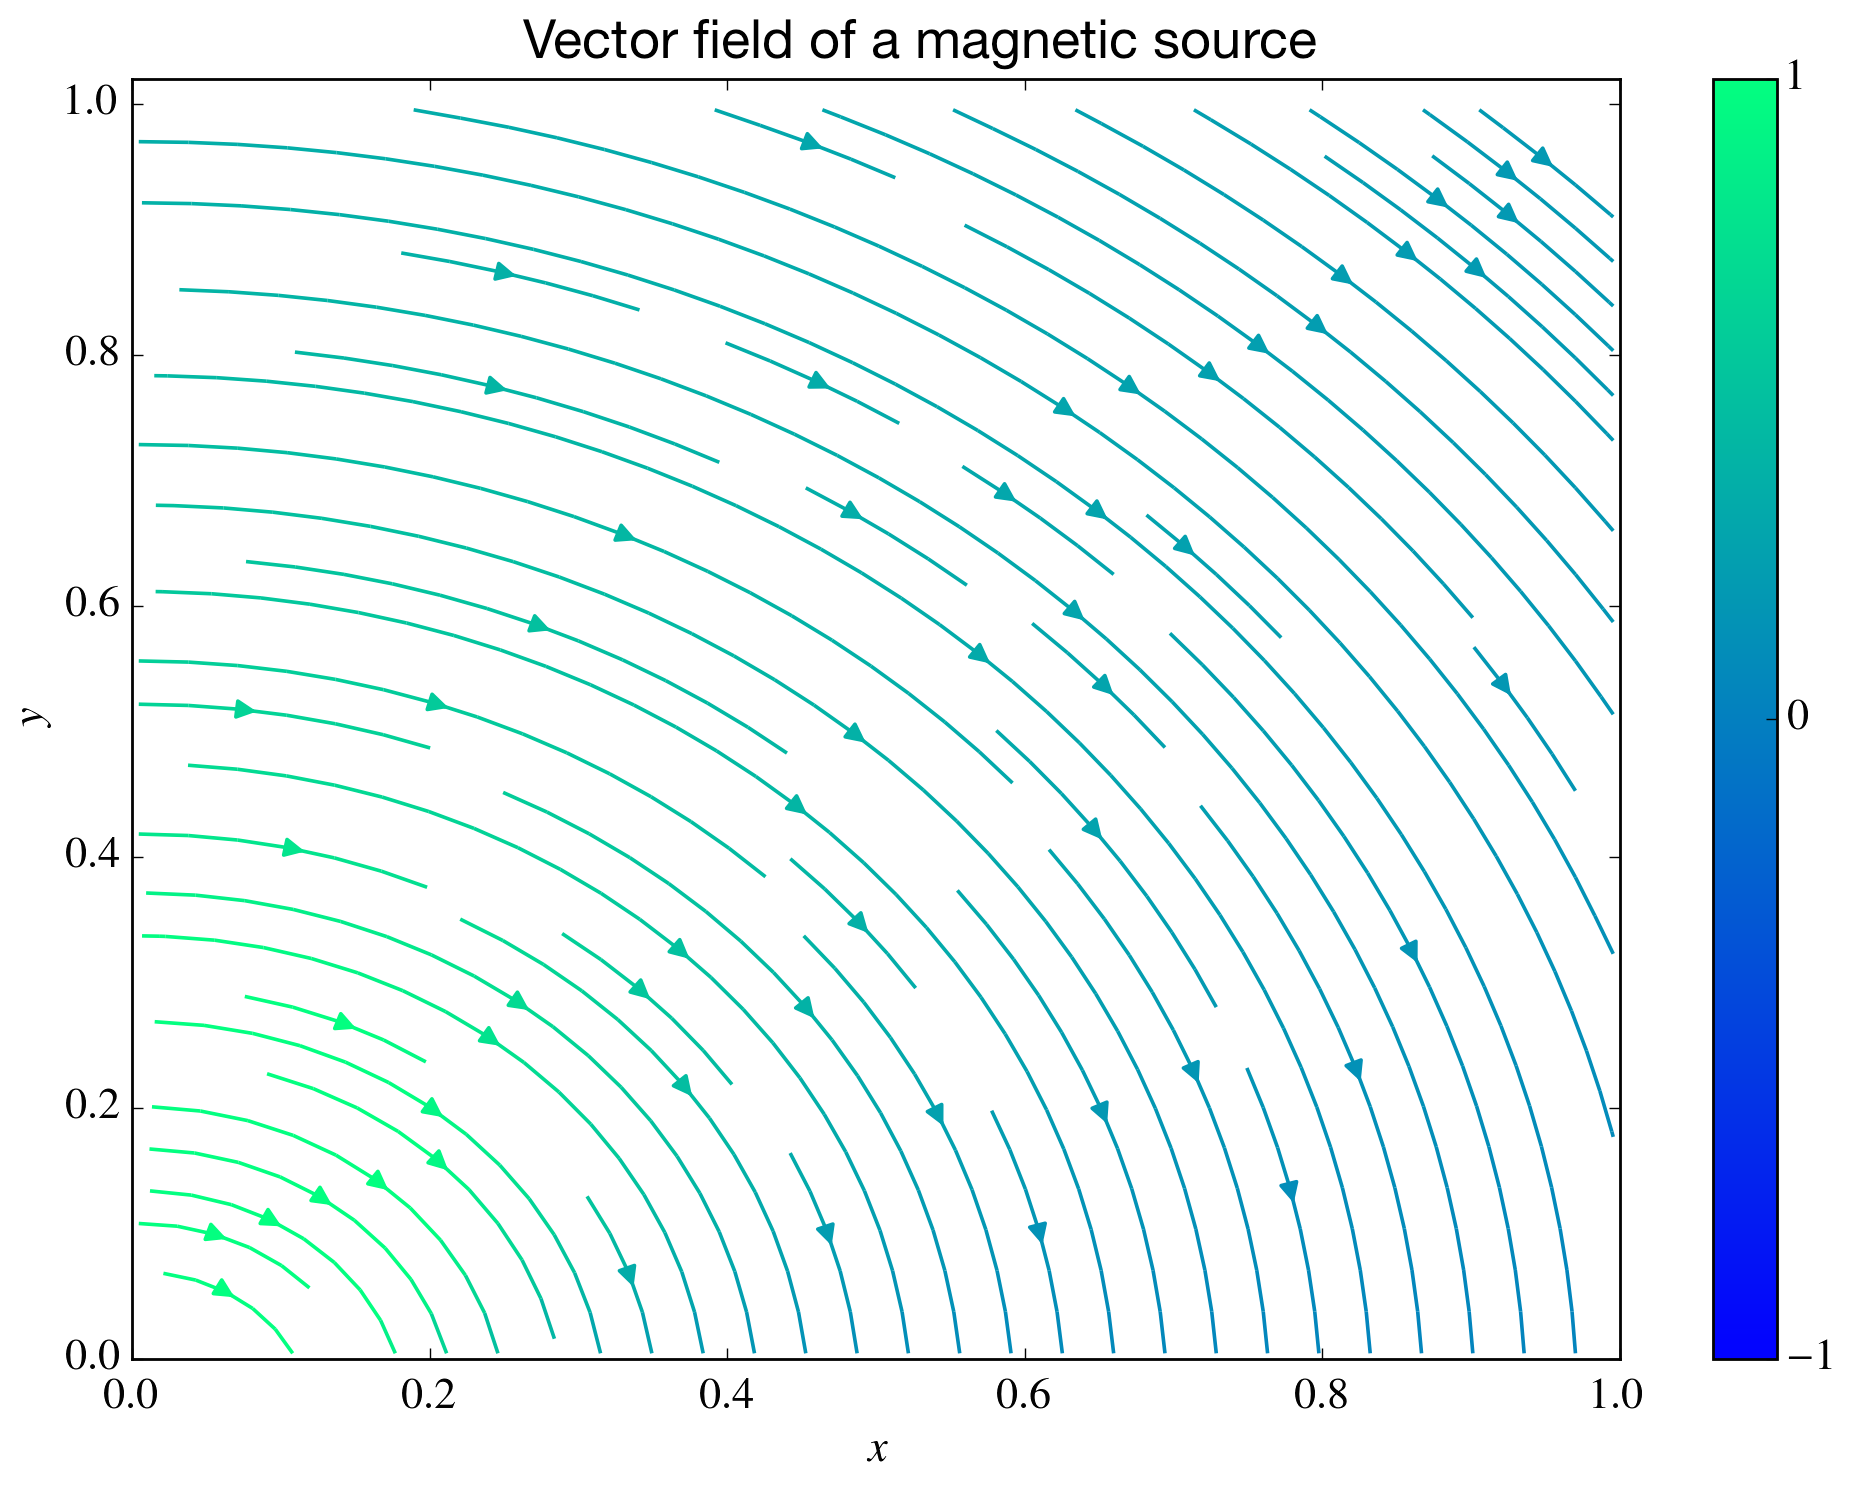
\includegraphics[width=\linewidth]{figures/vectorFieldH}
\caption{Applied magnetic field. All tests were made with this specific magnetic field. $\gamma$ values may change the actual intensity of field, but the streamlines are similar.\label{magneticField}}
\end{figure}


\begin{figure}[!t]
\centering
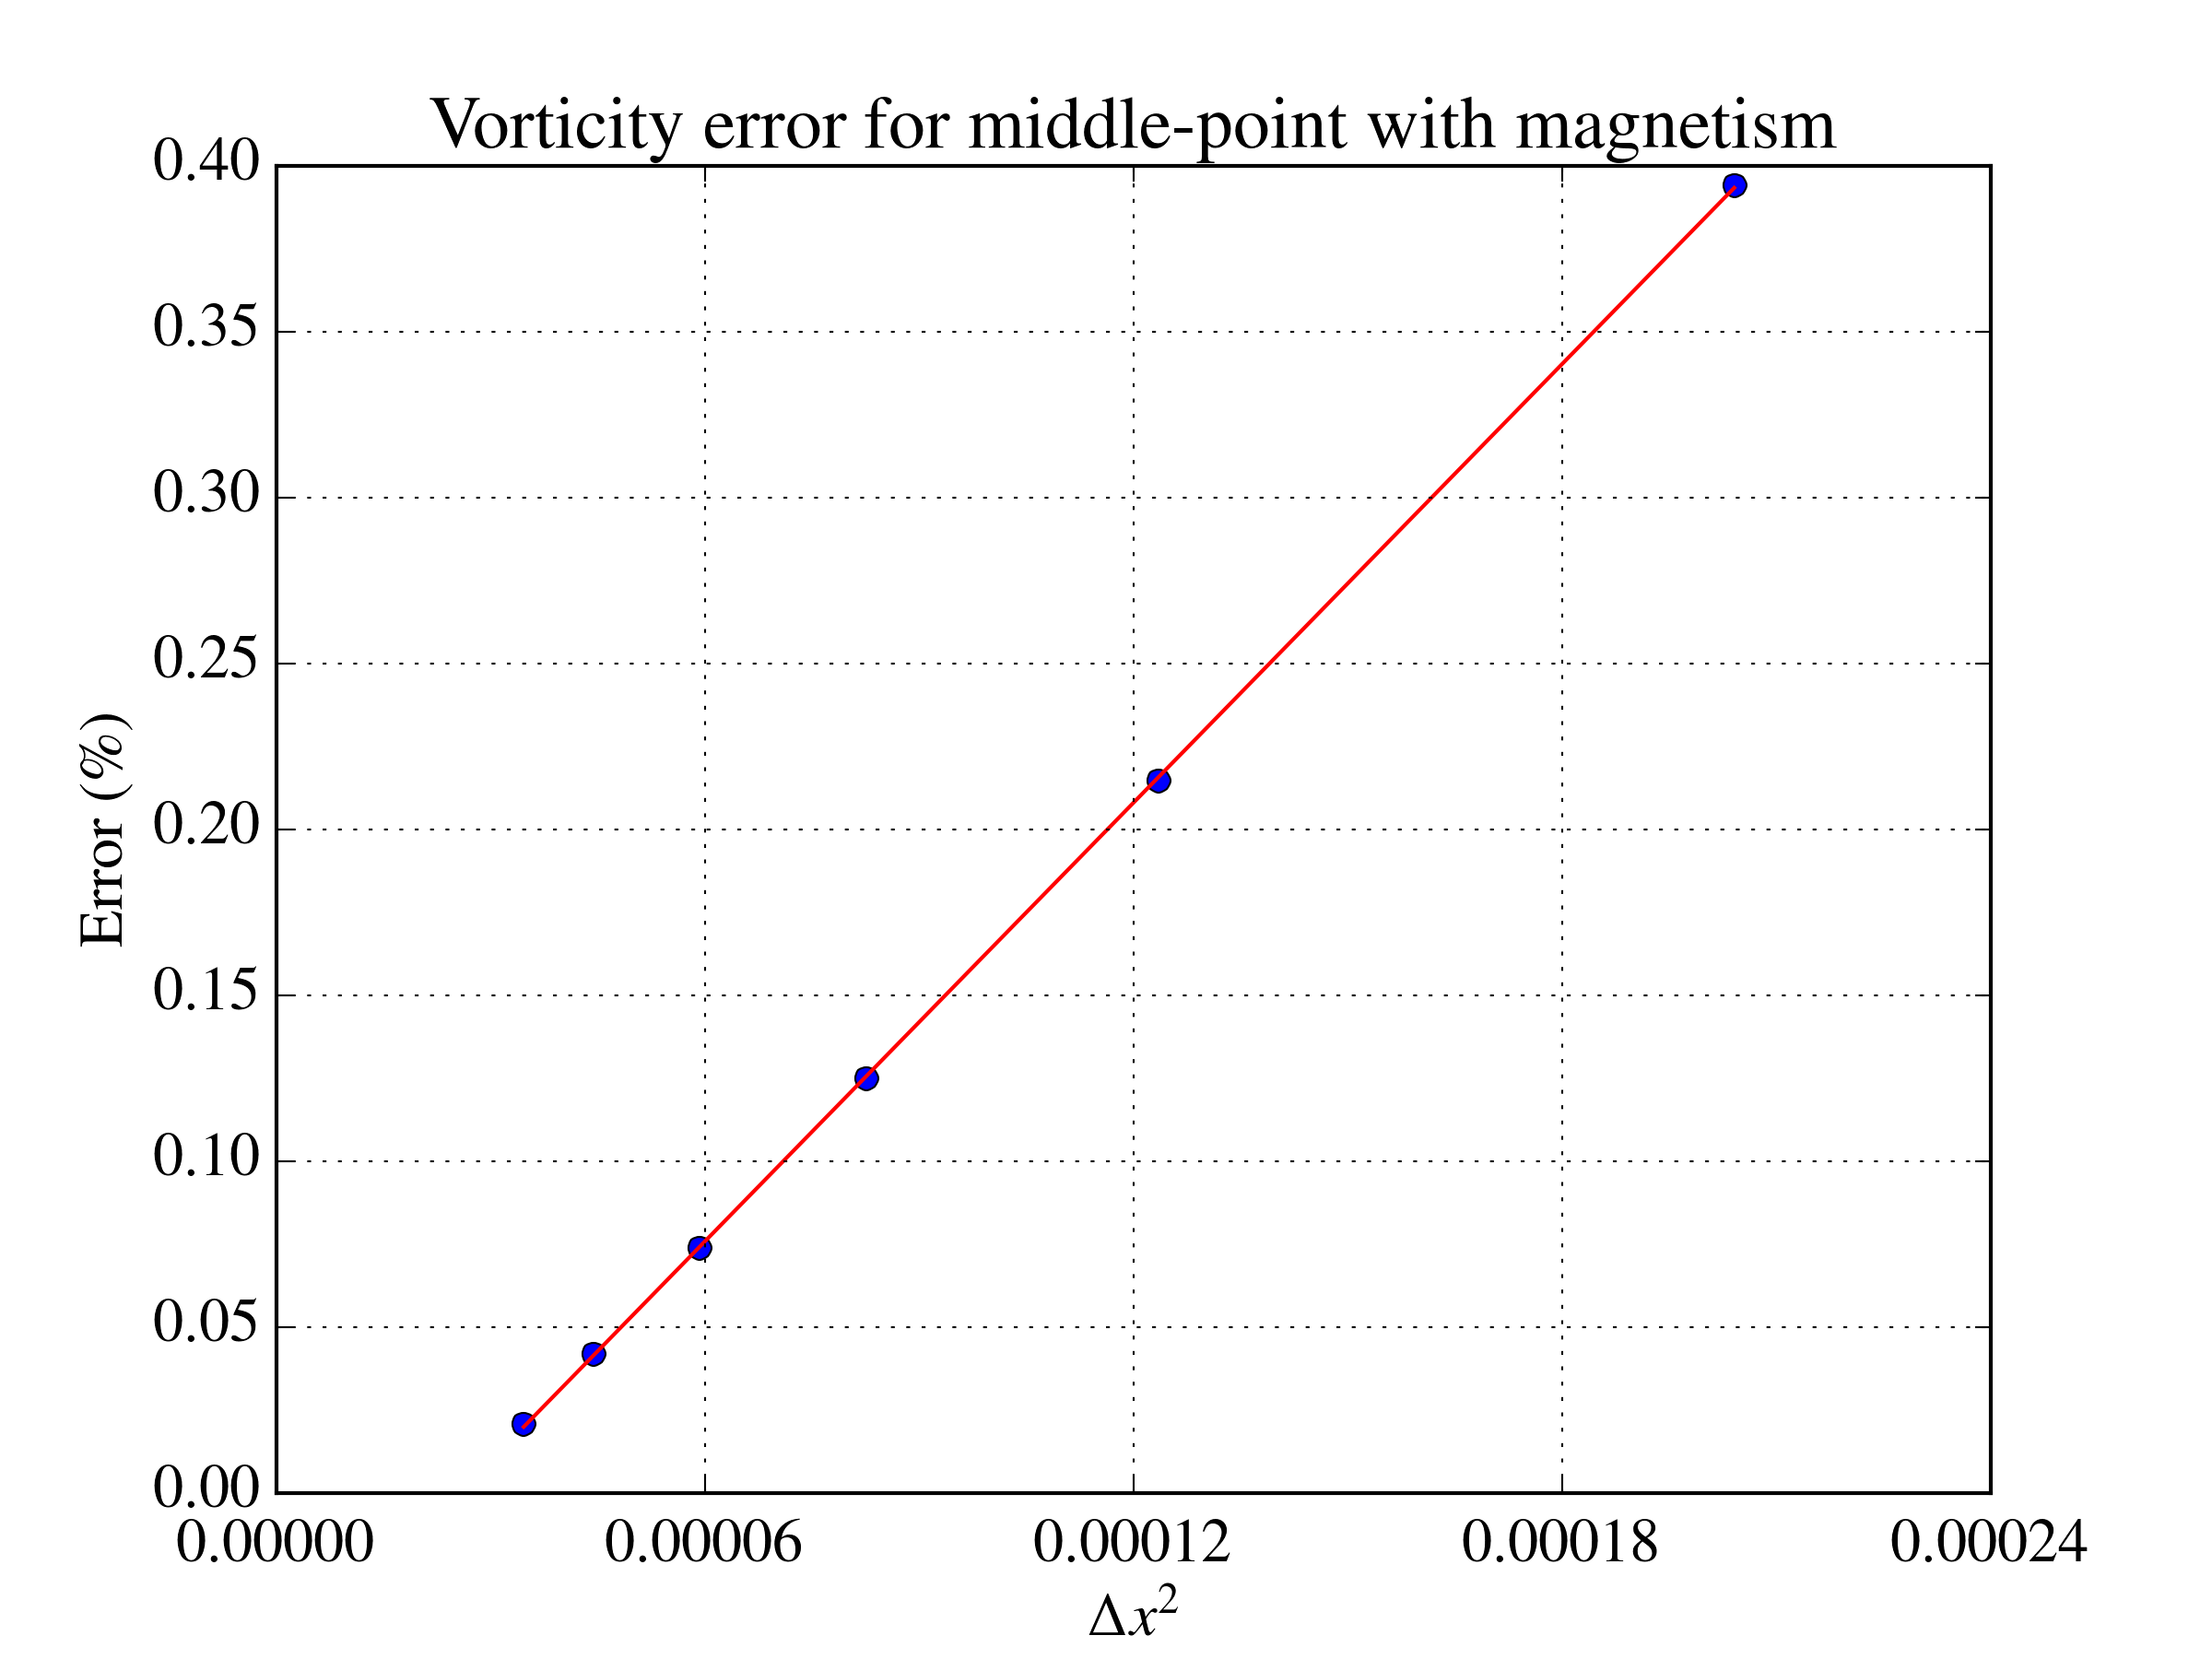
\includegraphics[width=\linewidth]{figures/validateMagnetismRe40}
\caption{Error evolving according to grid size. Higher grid sizes are closer to left-bottom corner. Error decays quadratically. Comparison with solution of $200\times 200$ grid. Grid sizes from $70\times 70$ to $170\times 170$. \label{magneticTest}}
\end{figure}



\subsection{Preliminary studies of flow patterns}
We have performed some tests to assess the influence of the dimensionless parameters $\mathit{Re}$ and $\mathrm{C}_\mathrm{pm}$ on the steady-state regimes that were obtained.  Some Reynolds numbers were chosen and then several tests were executed for some fixed magnetic parameters. The magnetic parameters are $\chi=0.5$, $\mathrm{C}_\mathrm{pm}=0.8$ and $\gamma=3.5$. Reynolds numbers presented here are 1, 50 and 100. Figures \ref{Re001nVectorField} to \ref{Re100wPressure} present streamlines for the velocity and contour lines for the pressure. Images with magnetic parameters set to 0 are the ones without magnetization. All results are in steady state. We have also coded a routine to calculate the angle between $\mathbf{M}$ and $\mathbf{H}$ for every point in those simulations but, for the case presented here, this is not relevant, as $\mathbf{M}=\chi\mathbf{H}$ is one consideration for the magnetization in the current work (superparamagnetic regime).

\begin{figure}[!t]
\centering
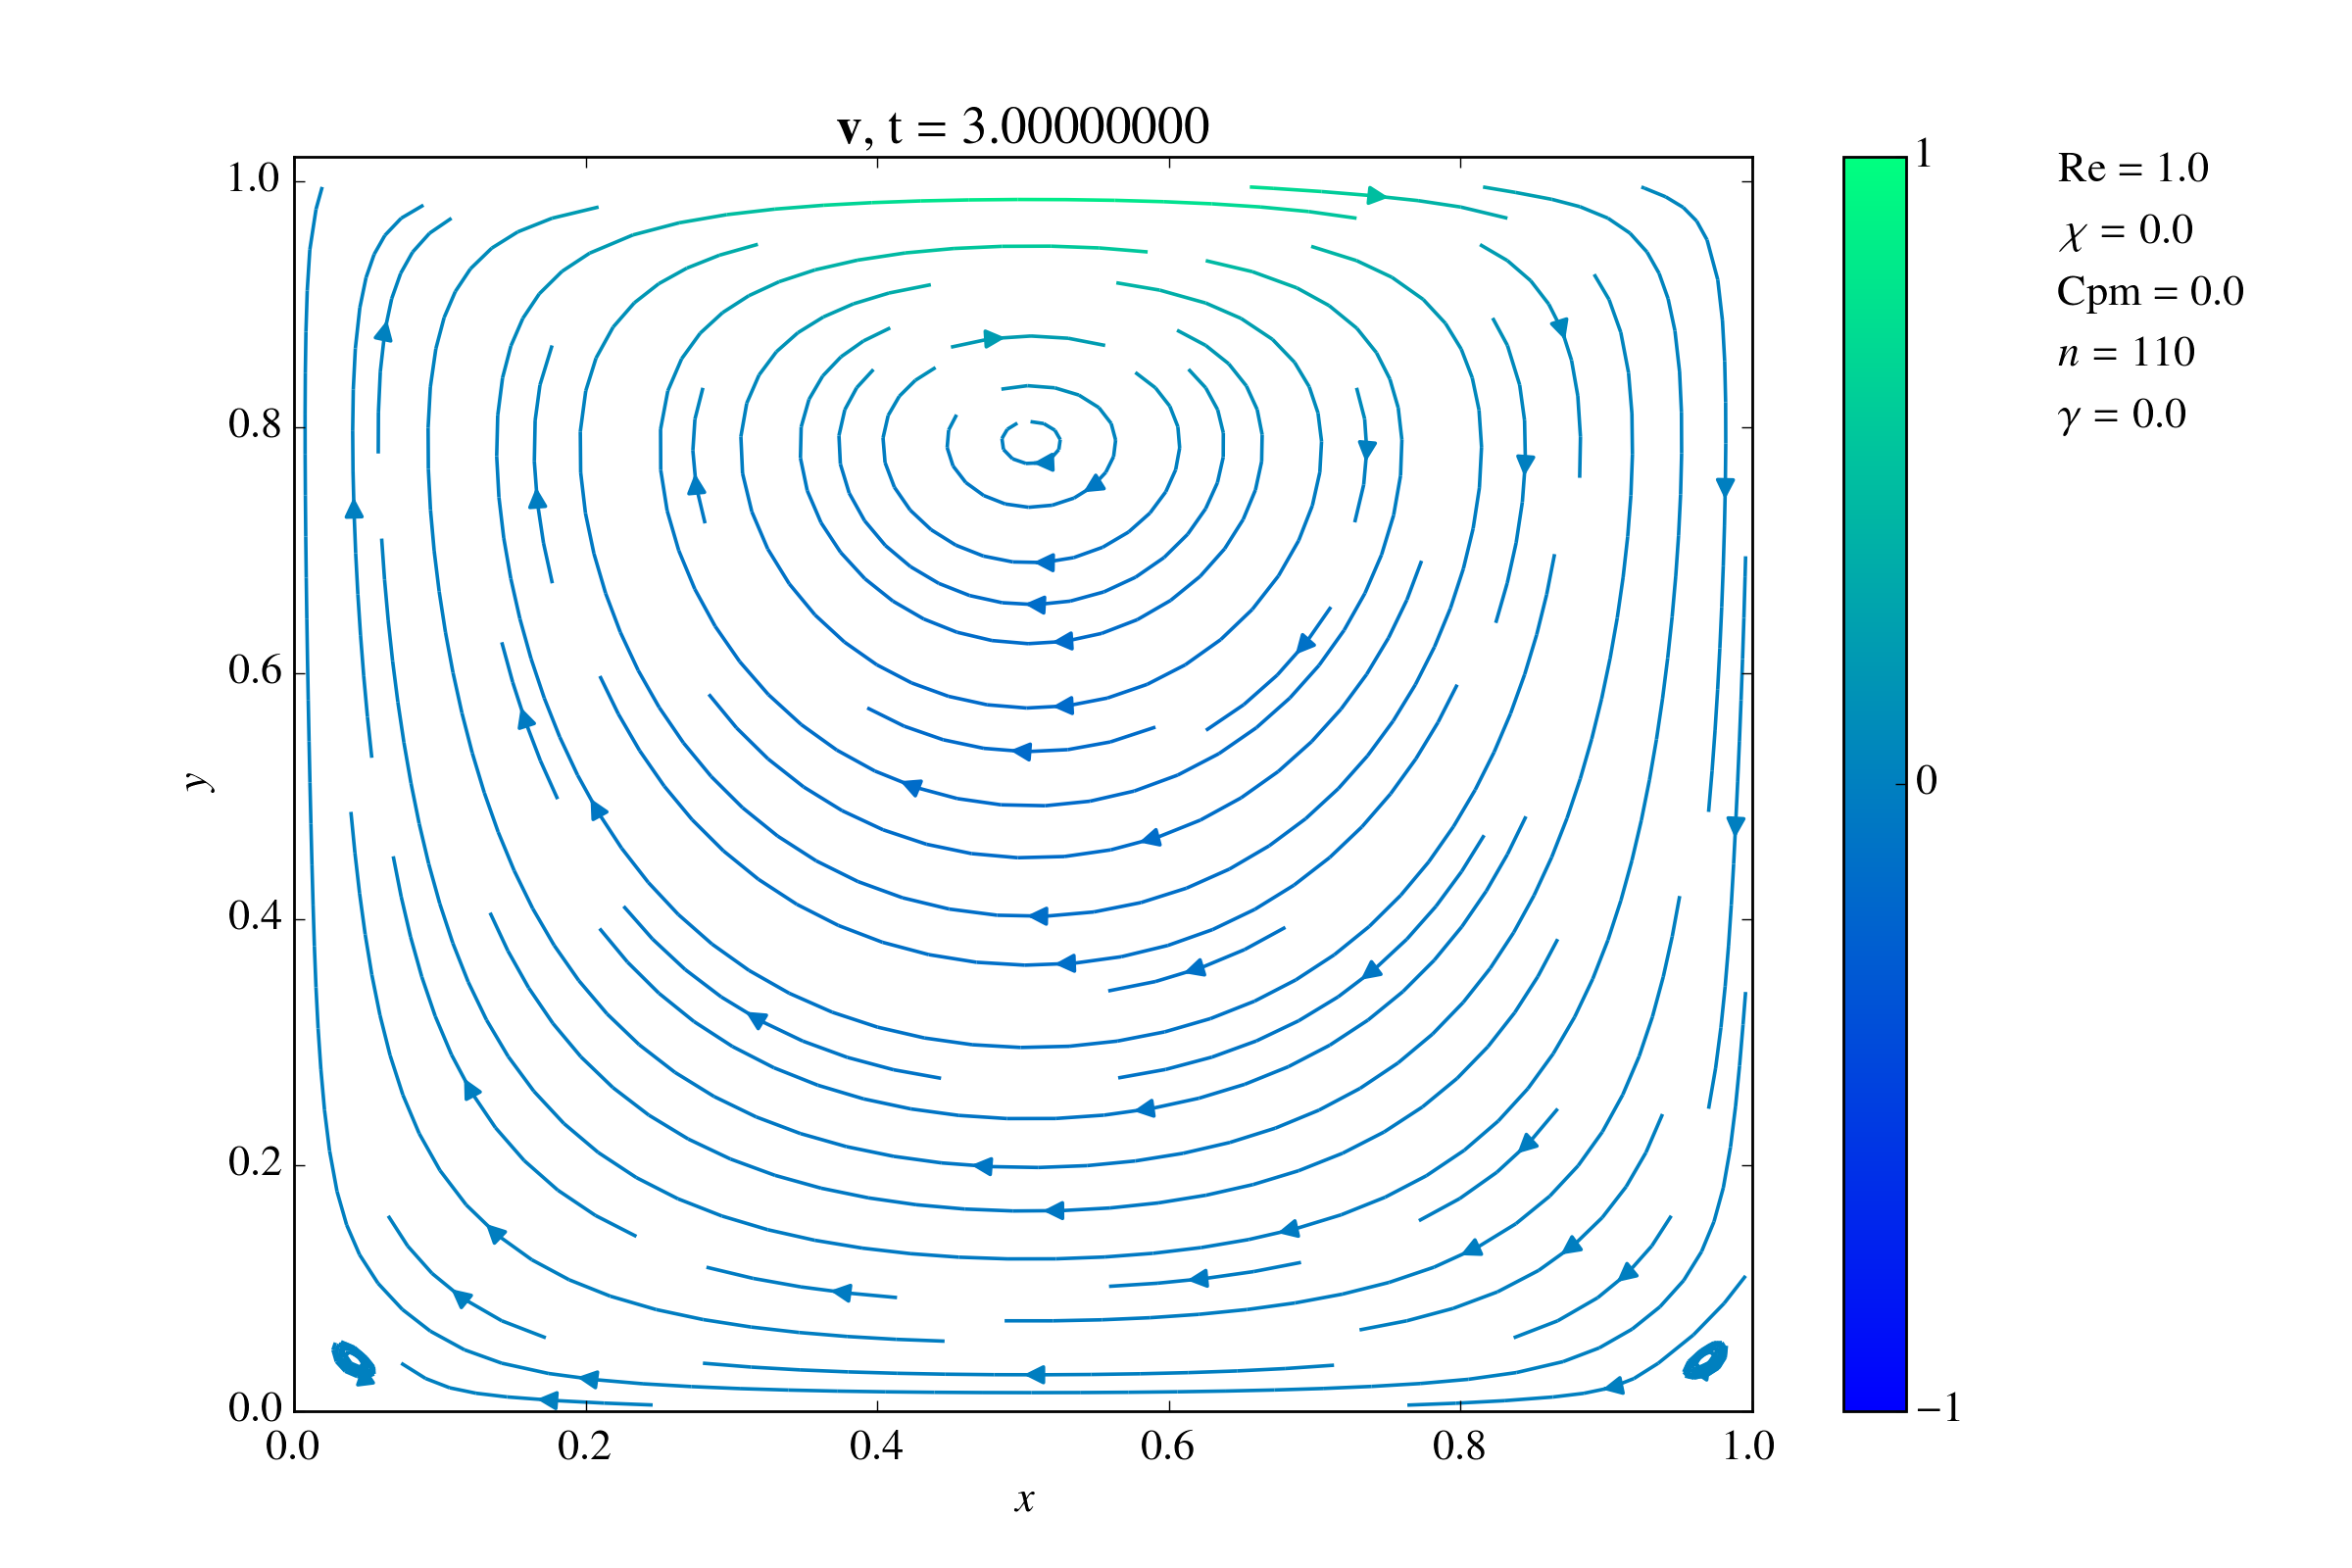
\includegraphics[width=\linewidth]{figures/Re001/n/vectorField}
\caption{Steady state solution without magnetic field, $\mathit{Re}=1$. No extra vortices appear.\label{Re001nVectorField}}
\end{figure}

\begin{figure}[!t]
\centering
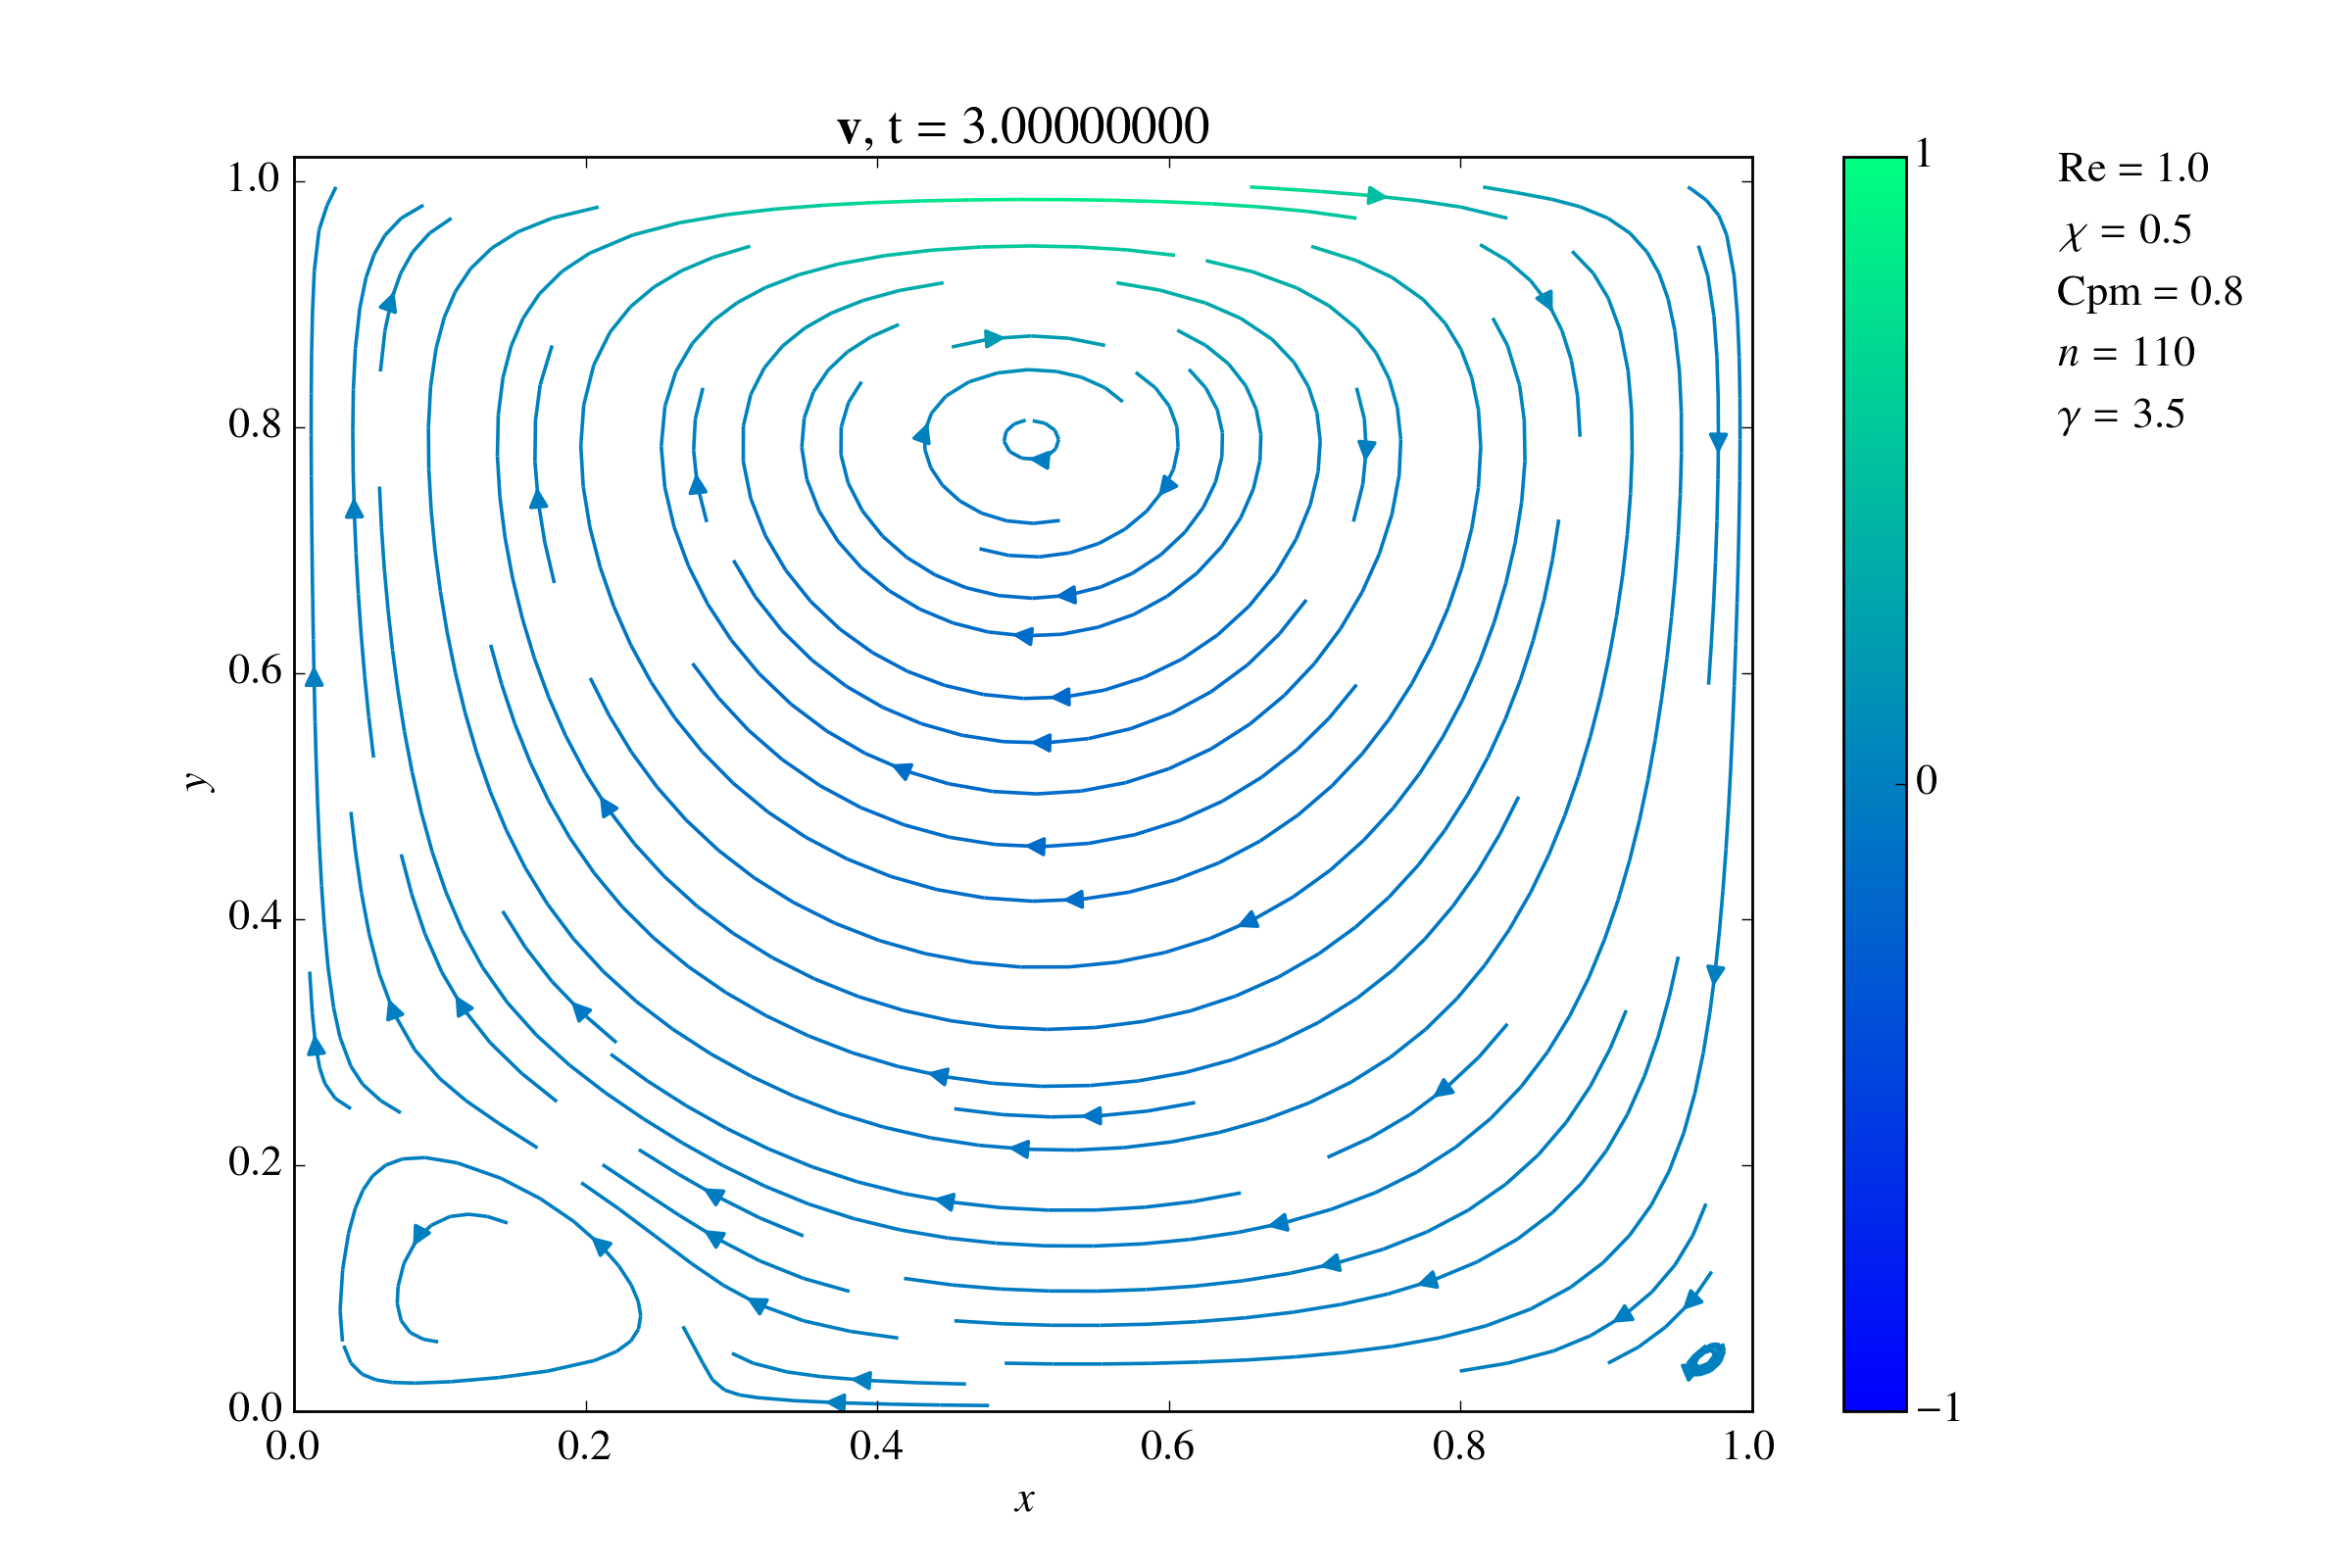
\includegraphics[width=\linewidth]{figures/Re001/w/vectorField}
\caption{Steady state solution without magnetic field, $\mathit{Re}=1$. A new vortex starts to appear. \label{Re001wVectorField}}
\end{figure}

\begin{figure}[!t]
\centering
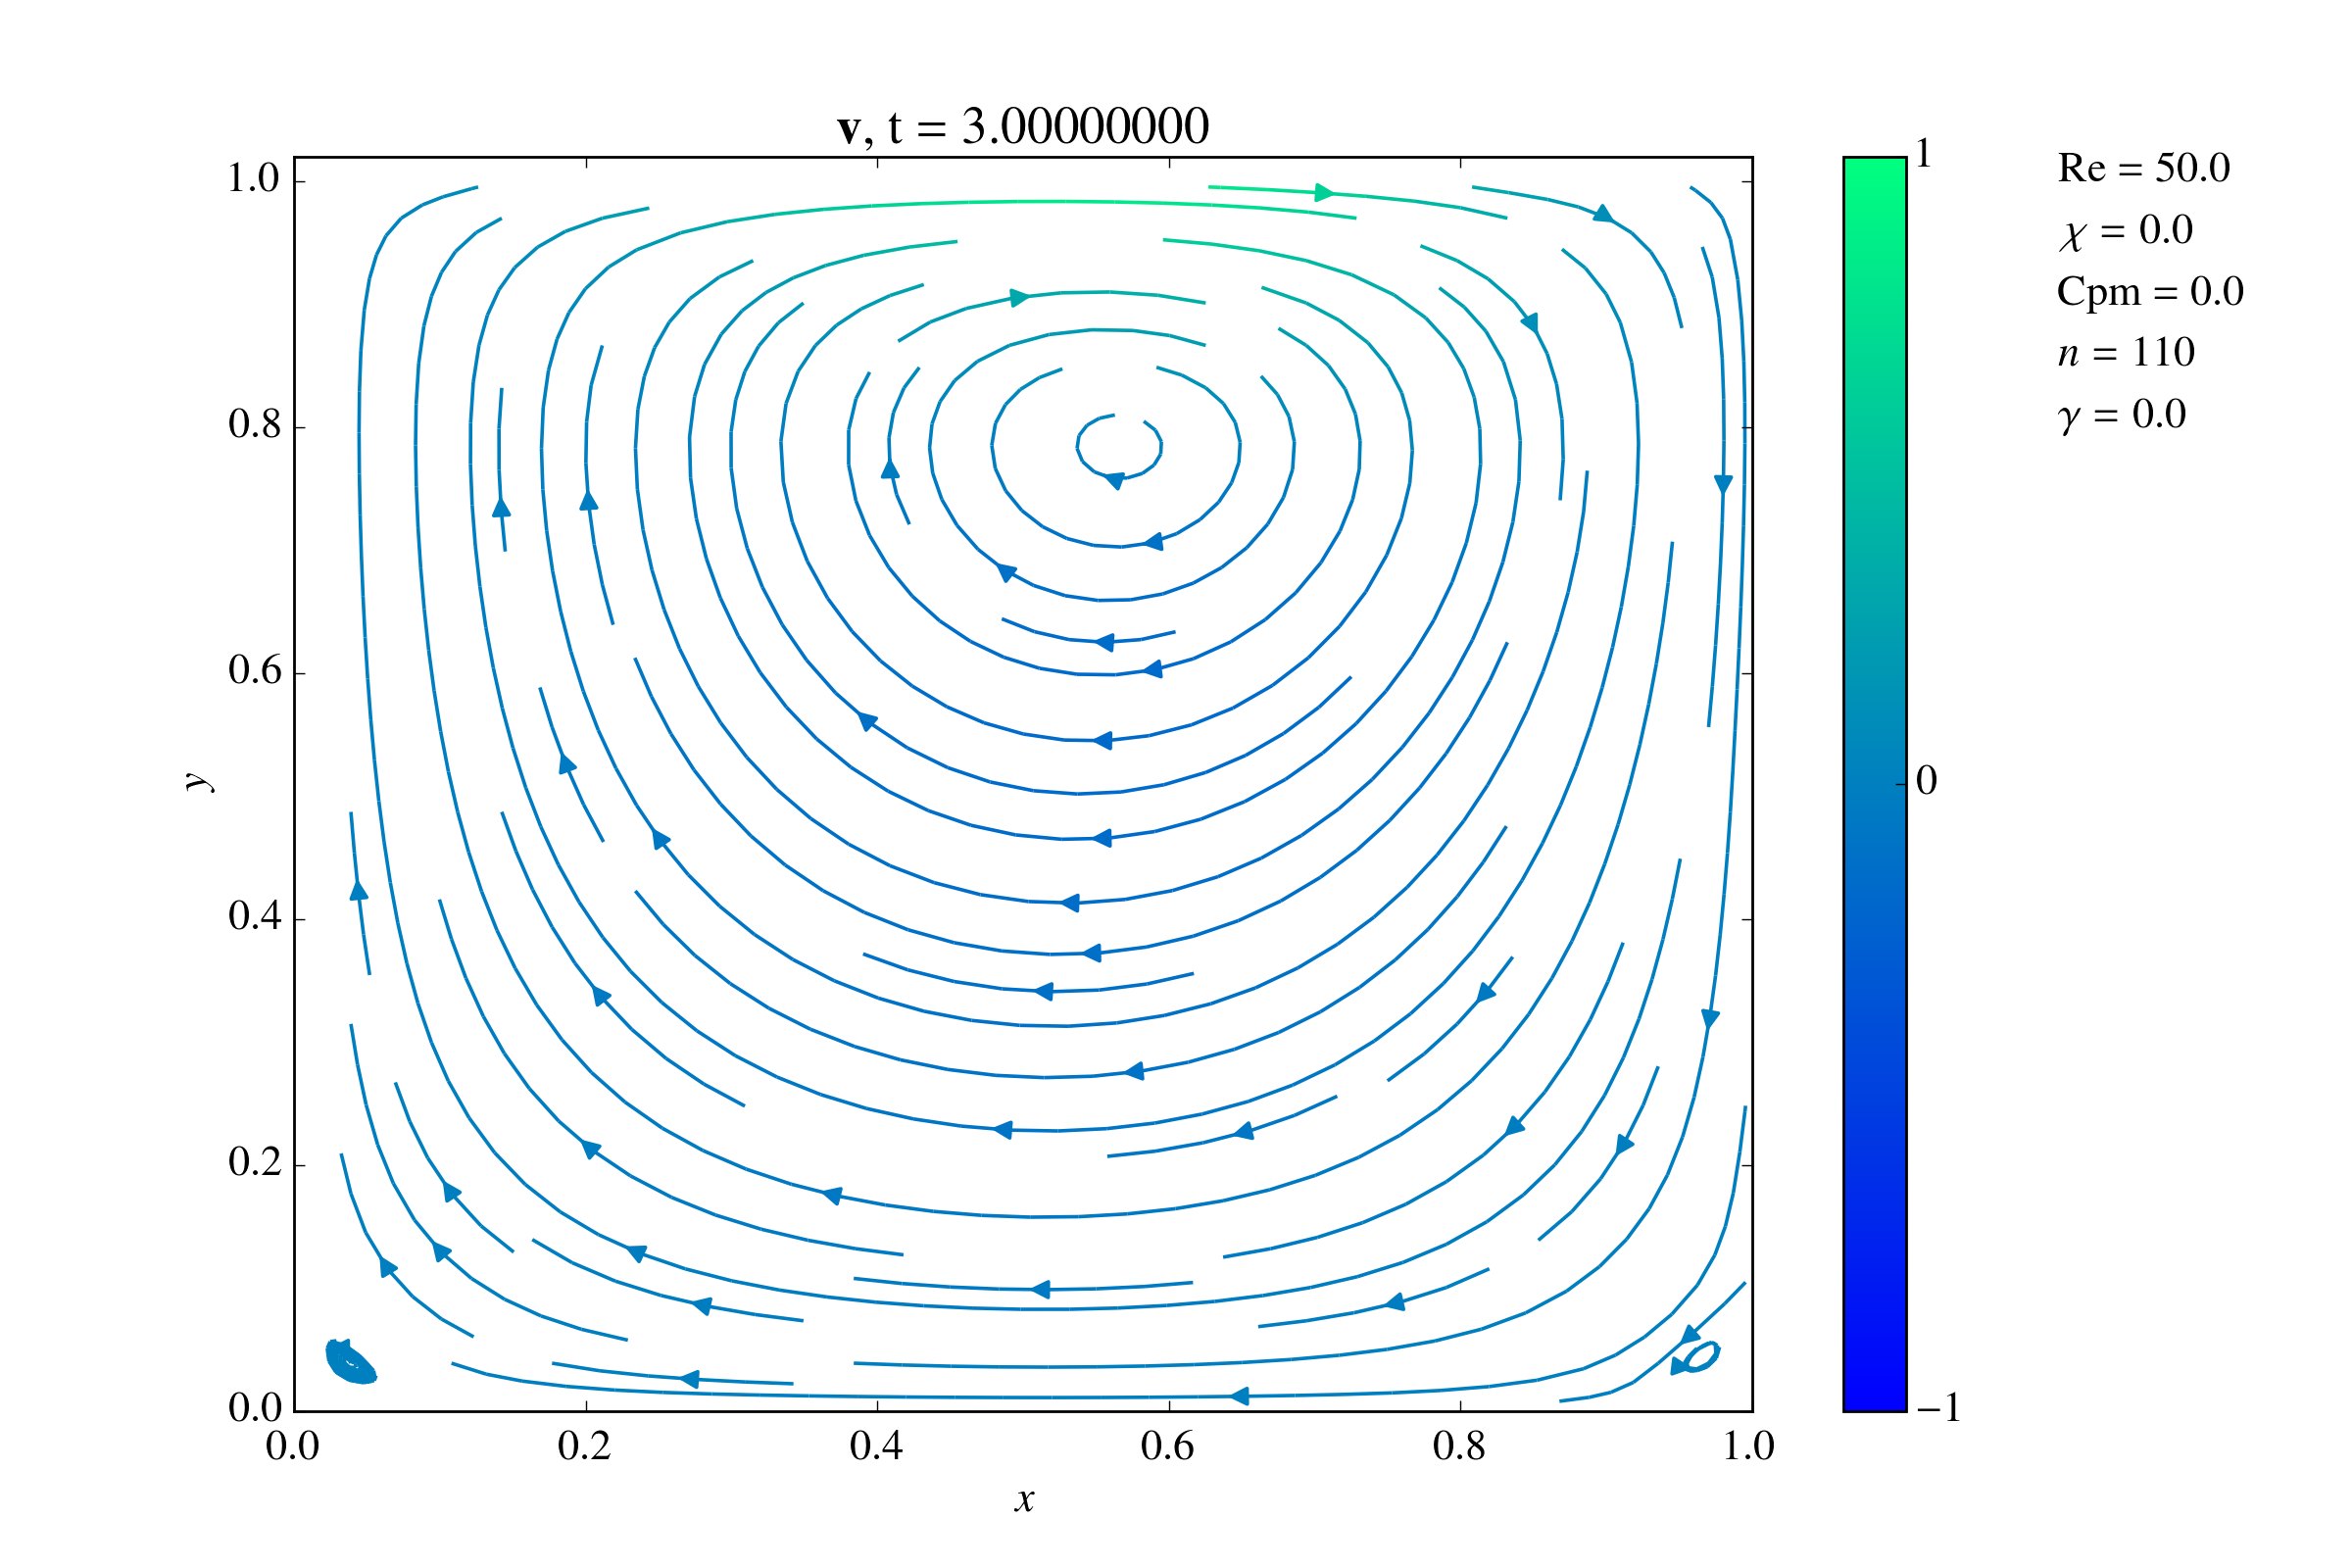
\includegraphics[width=\linewidth]{figures/Re050/n/vectorField}
\caption{Steady state solution without magnetic field, $\mathit{Re}=50$. No extra vortices appear. \label{Re050nVectorField}}
\end{figure}

\begin{figure}[!t]
\centering
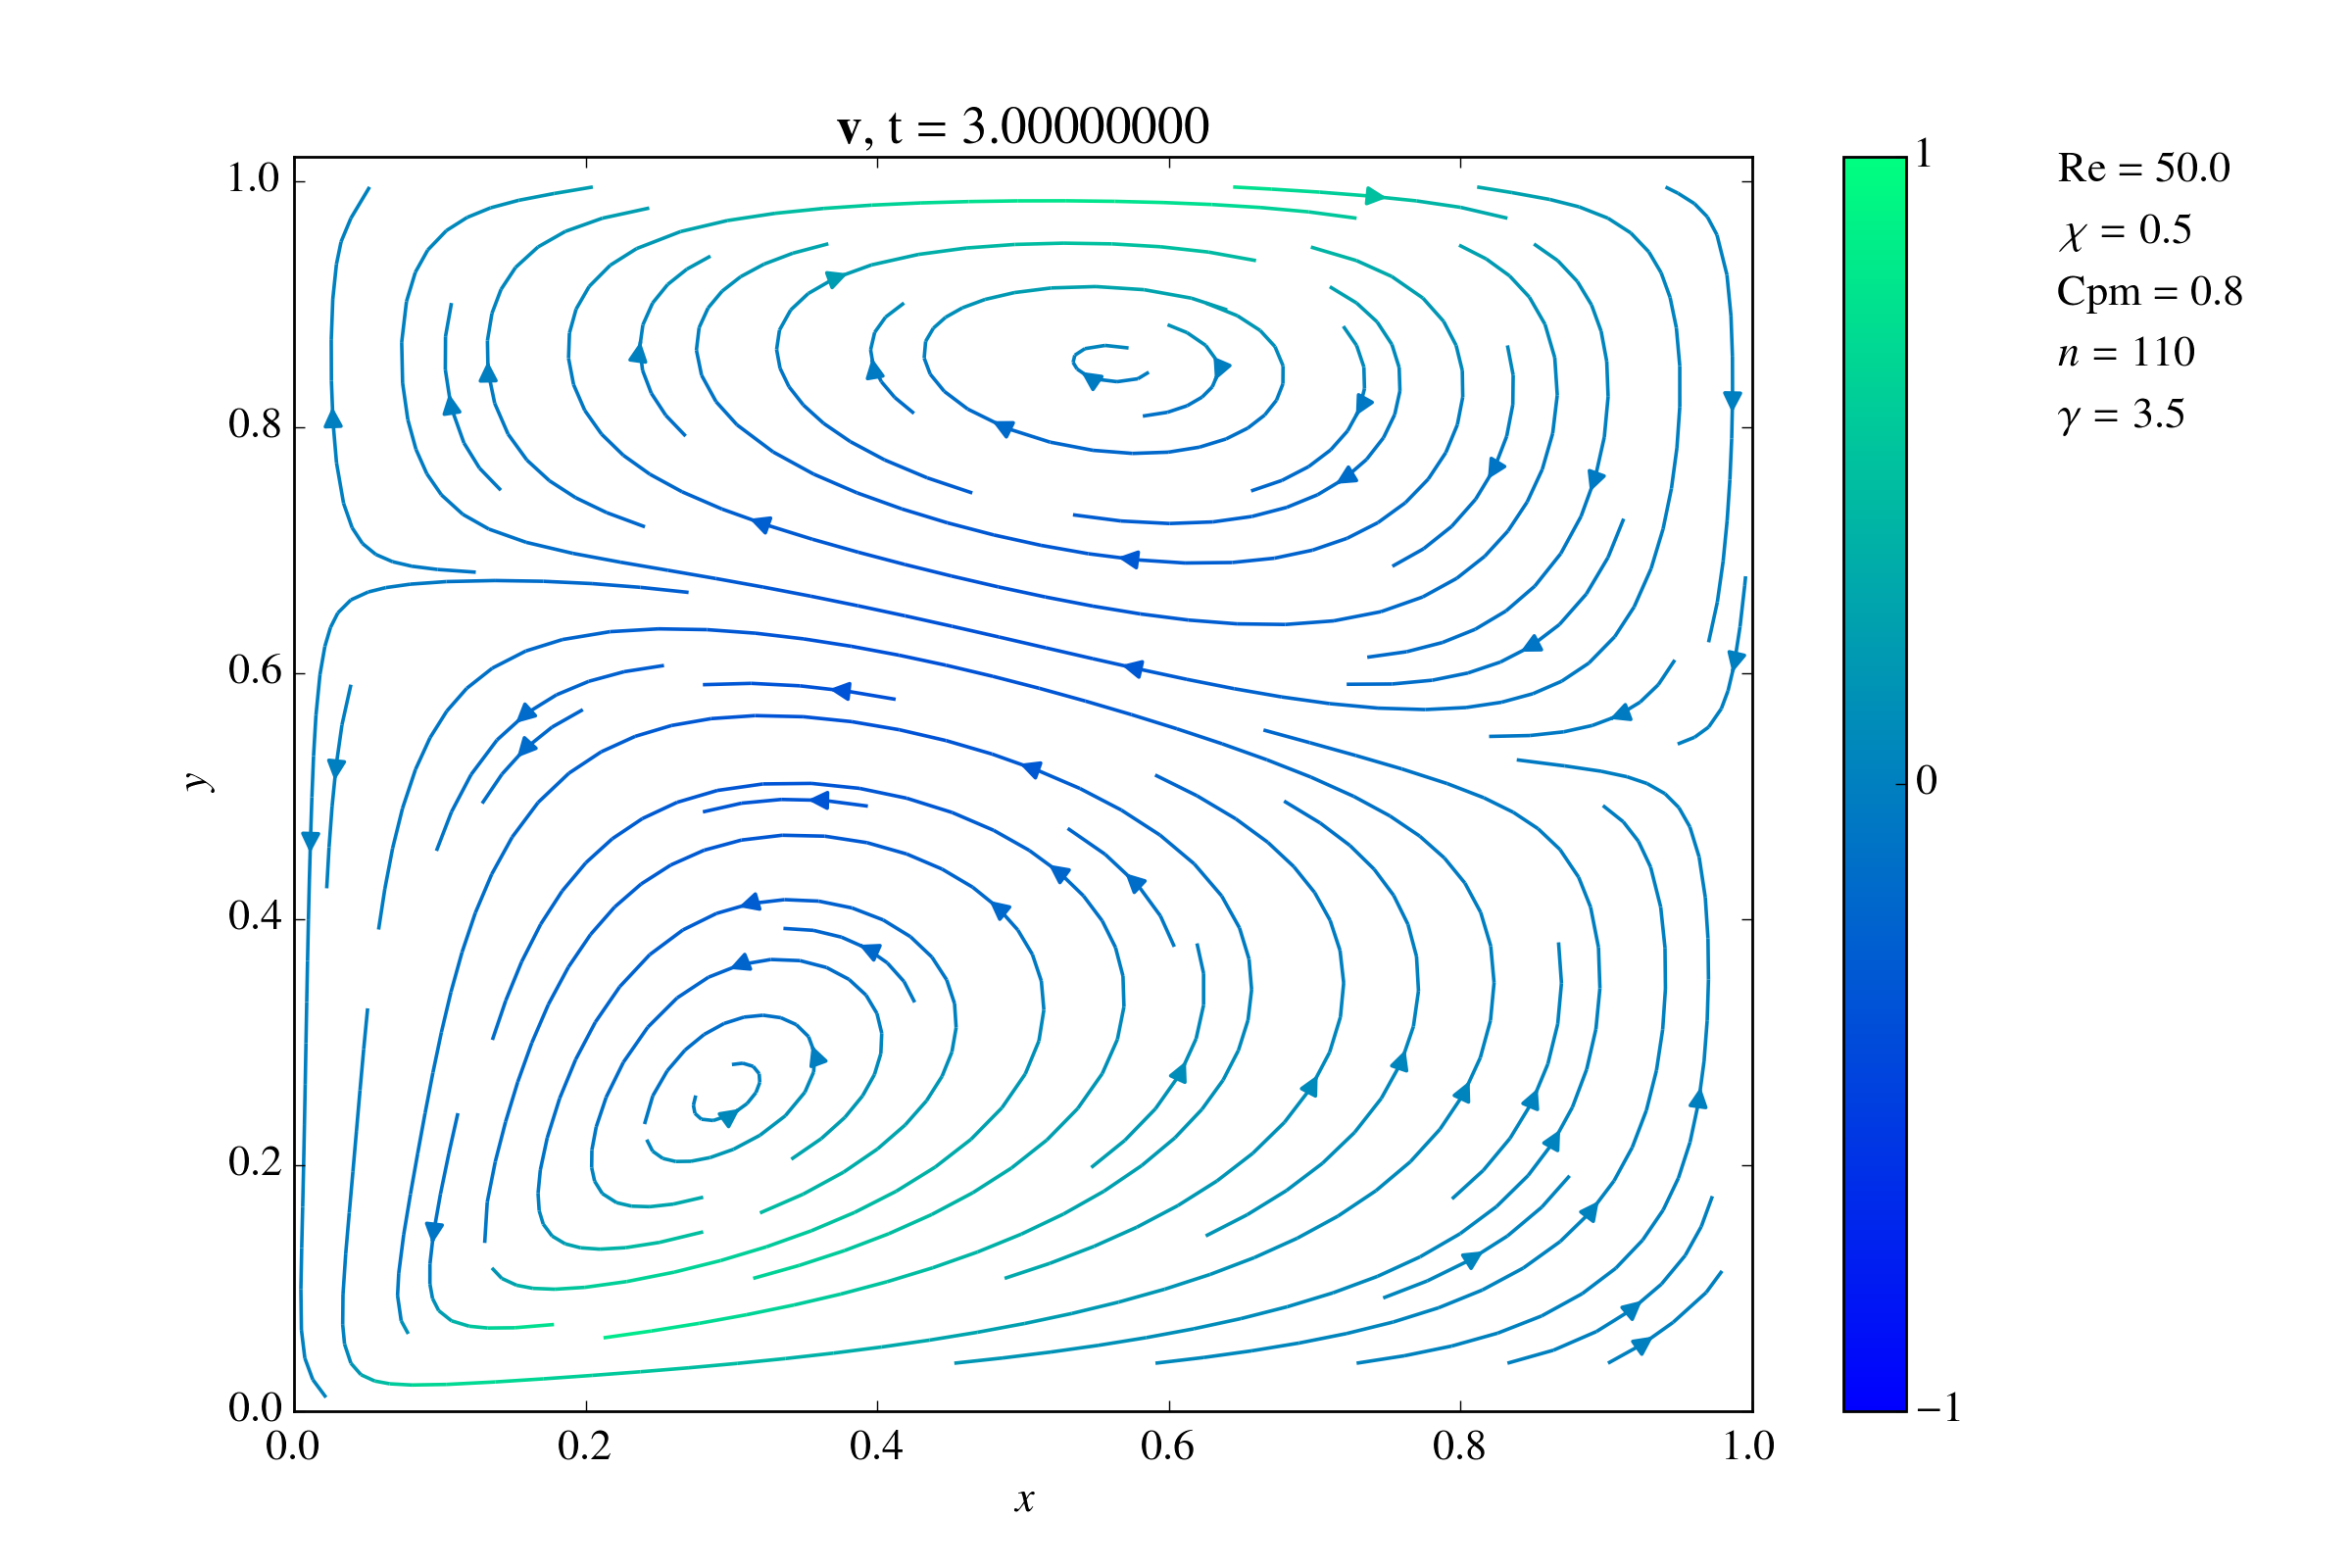
\includegraphics[width=\linewidth]{figures/Re050/w/vectorField}
\caption{Steady state solution without magnetic field, $\mathit{Re}=50$. The new vortex is already bigger than the initial one. \label{Re050wVectorField}}
\end{figure}

\begin{figure}[!t]
\centering
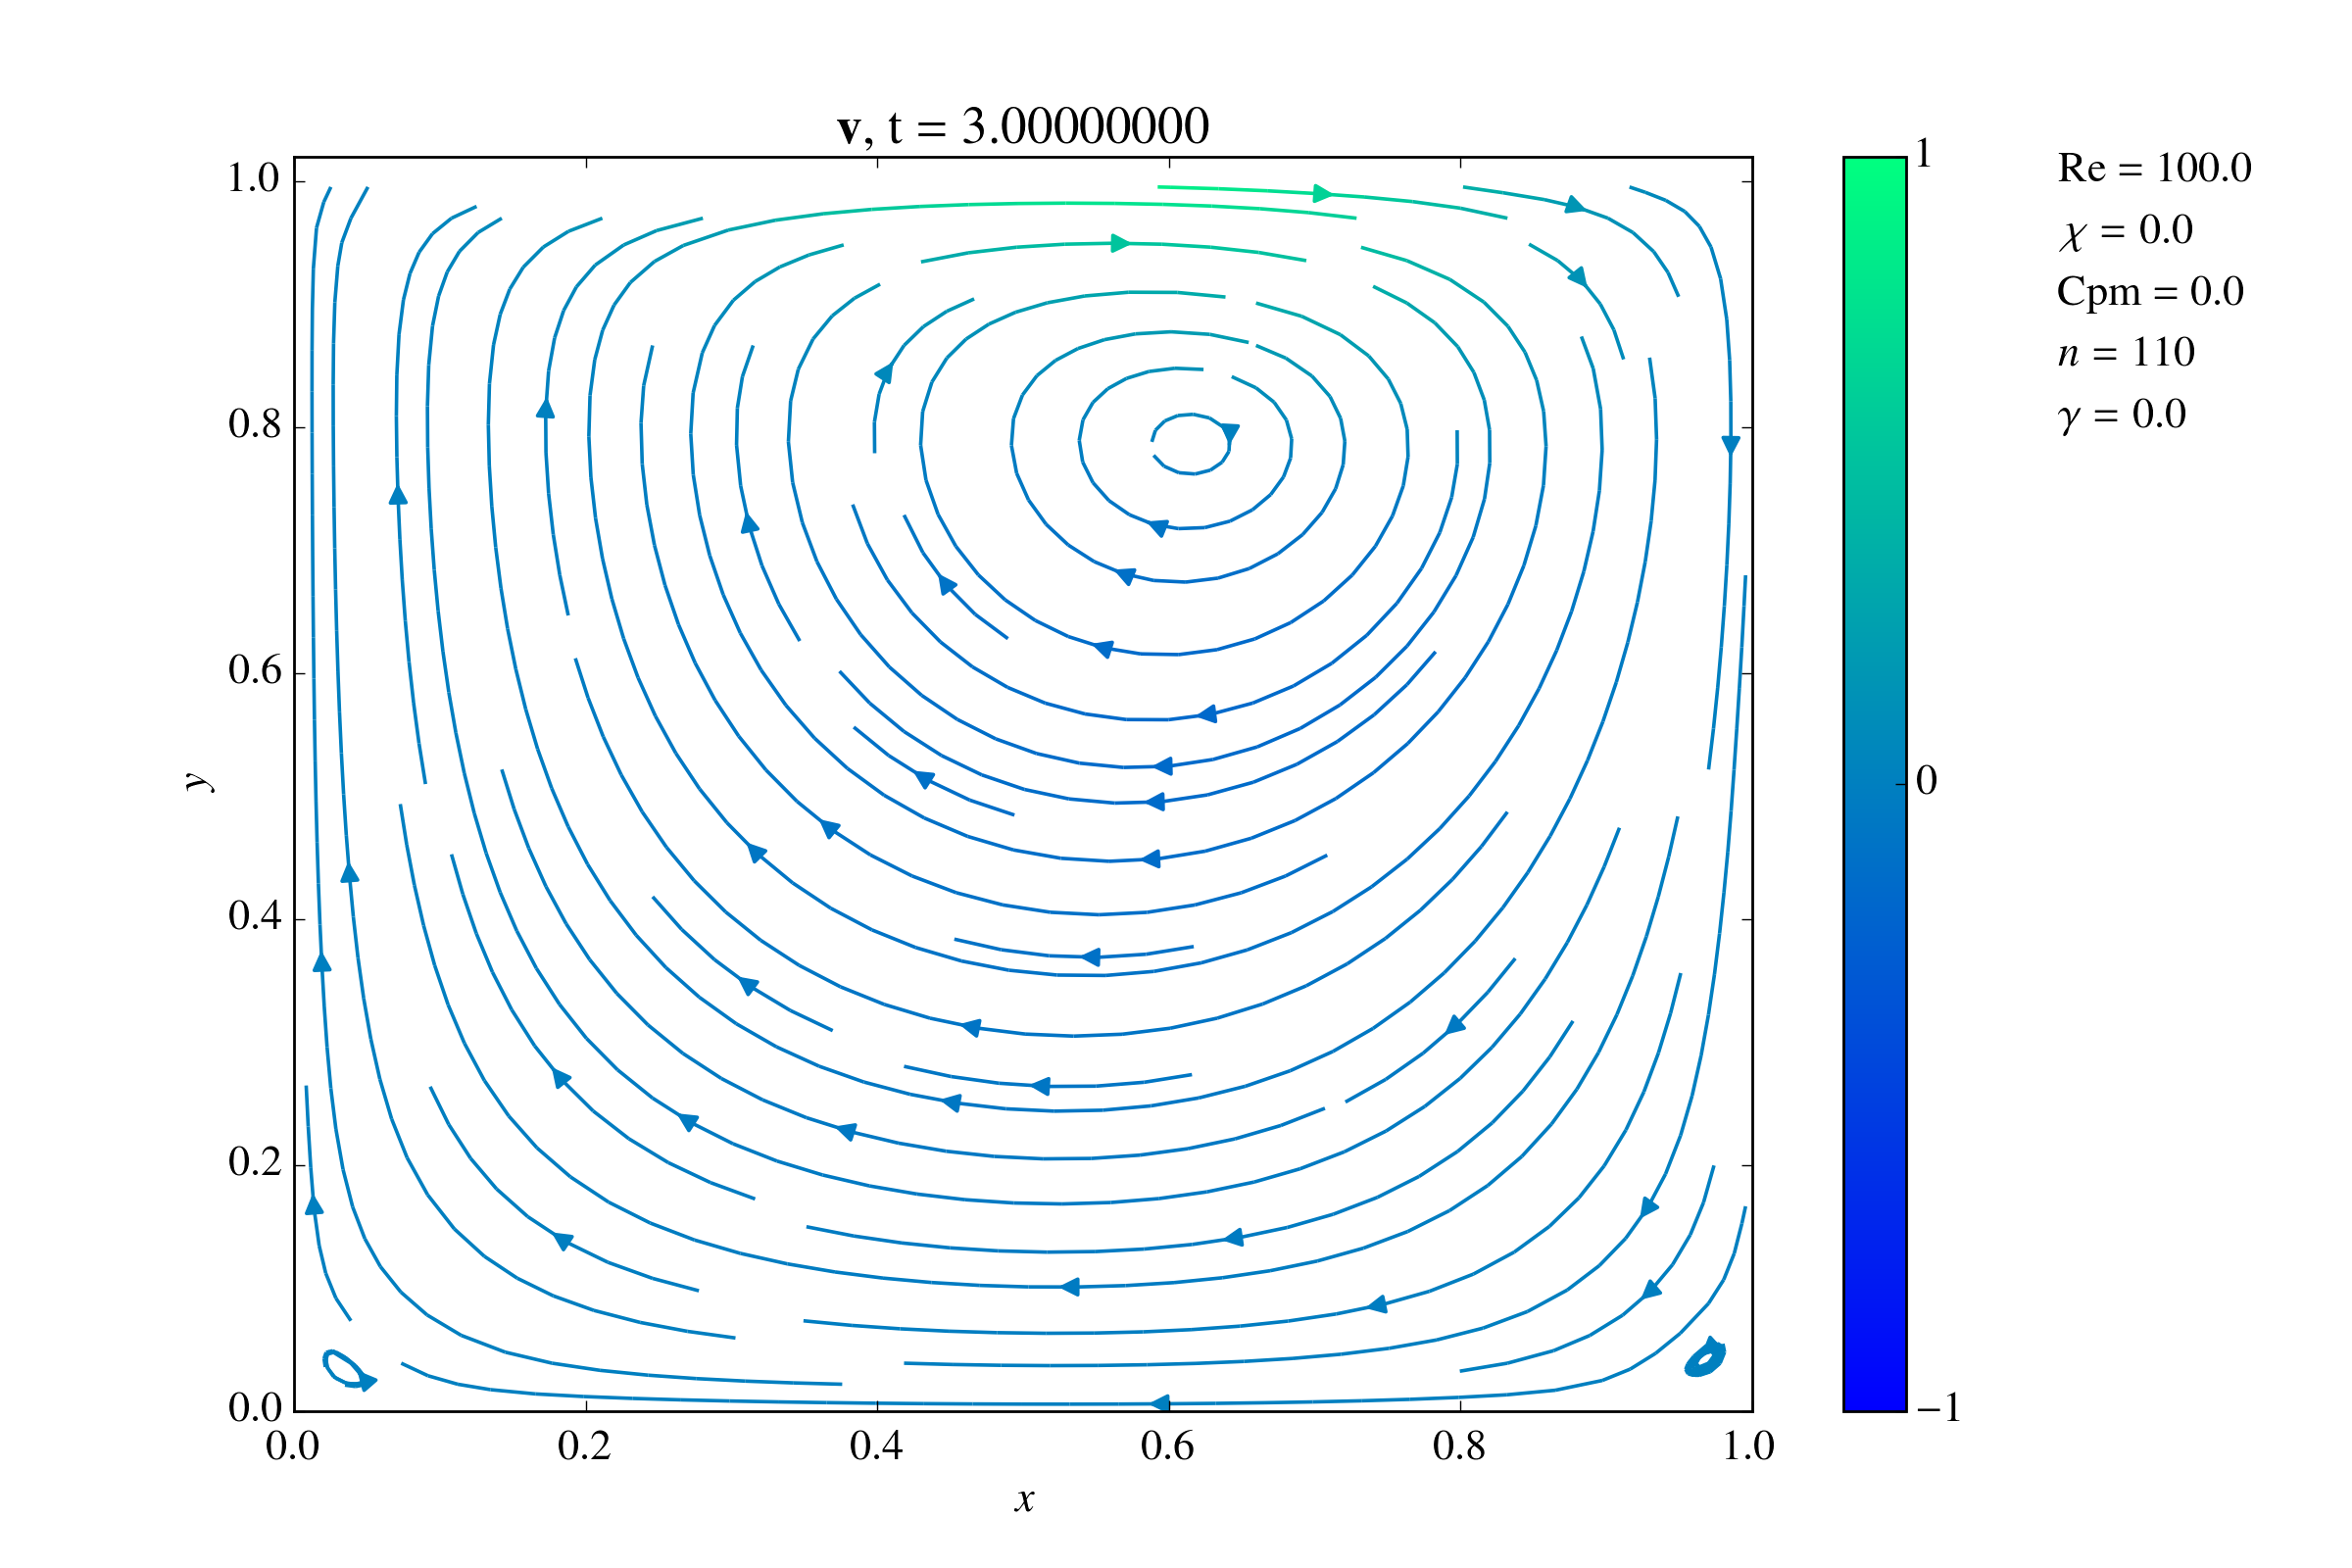
\includegraphics[width=\linewidth]{figures/Re100/n/vectorField}
\caption{Steady state solution without magnetic field, $\mathit{Re}=100$. No extra vortices appear. \label{Re100nVectorField}}
\end{figure}

\begin{figure}[!t]
\centering
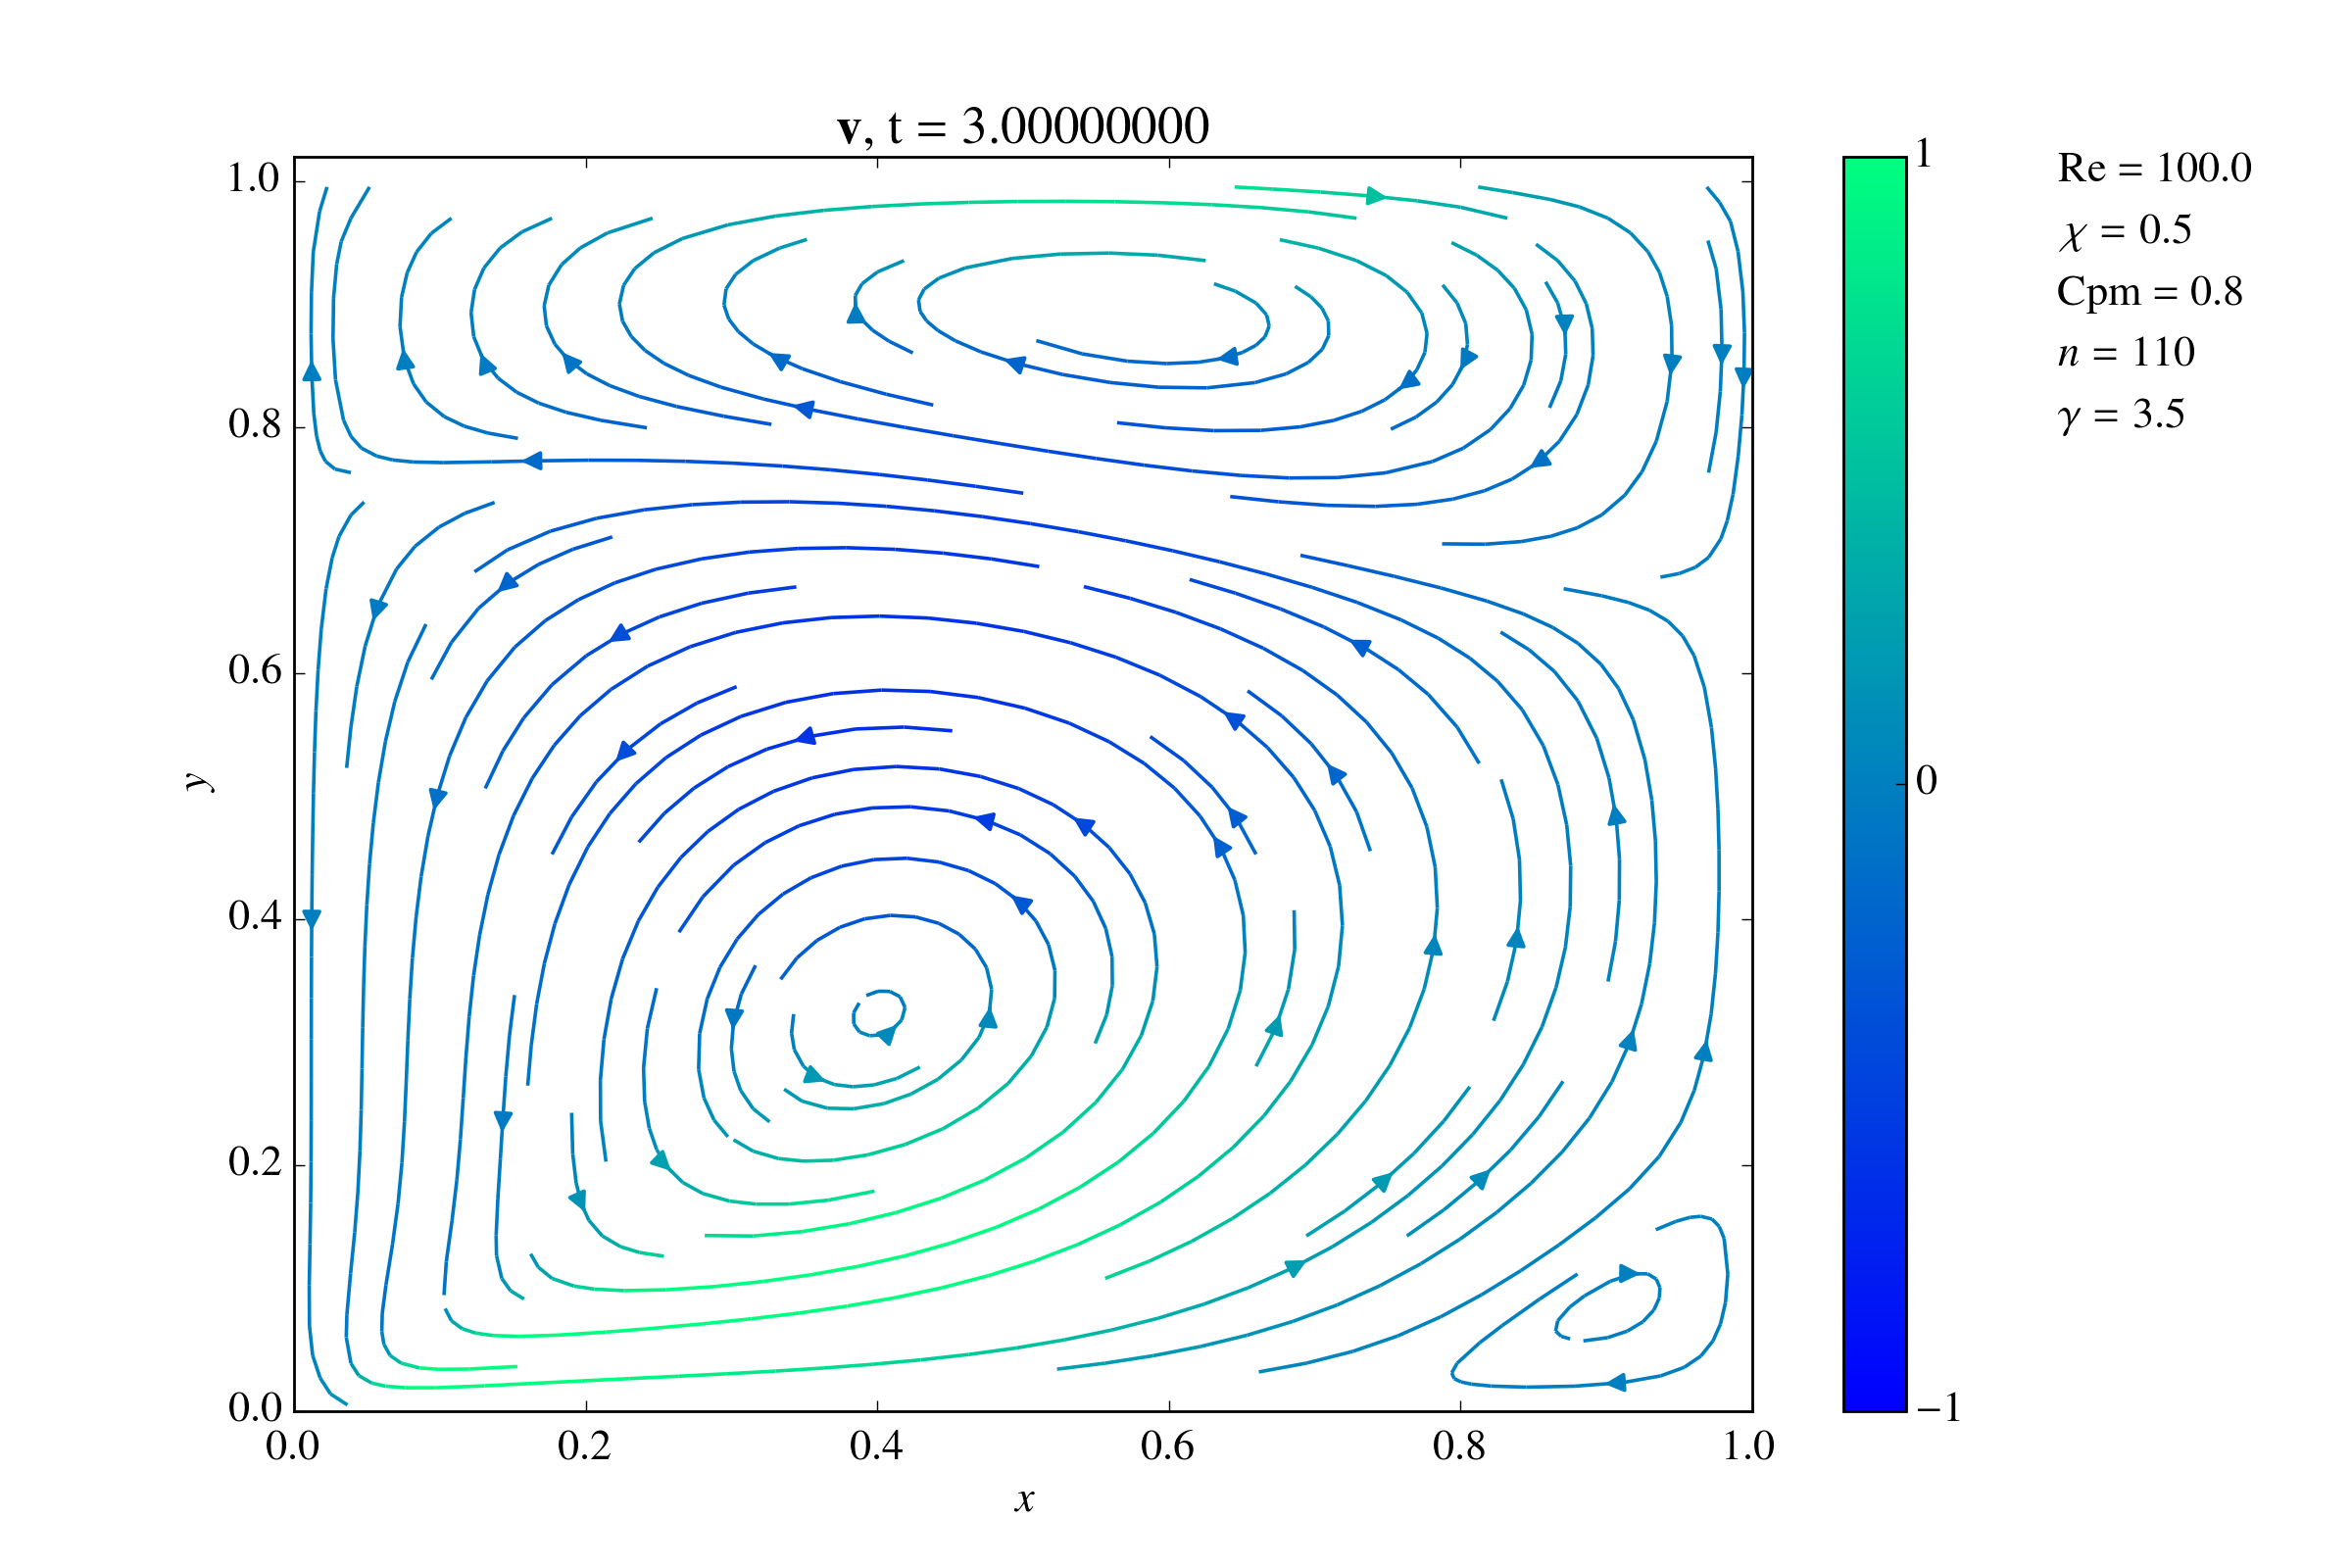
\includegraphics[width=\linewidth]{figures/Re100/w/vectorField}
\caption{Steady state solution without magnetic field, $\mathit{Re}=100$. Vortex increased in comparison with $\mathit{Re} = 50$. \label{Re100wVectorField}}
\end{figure}


\begin{figure}[!t]
\centering
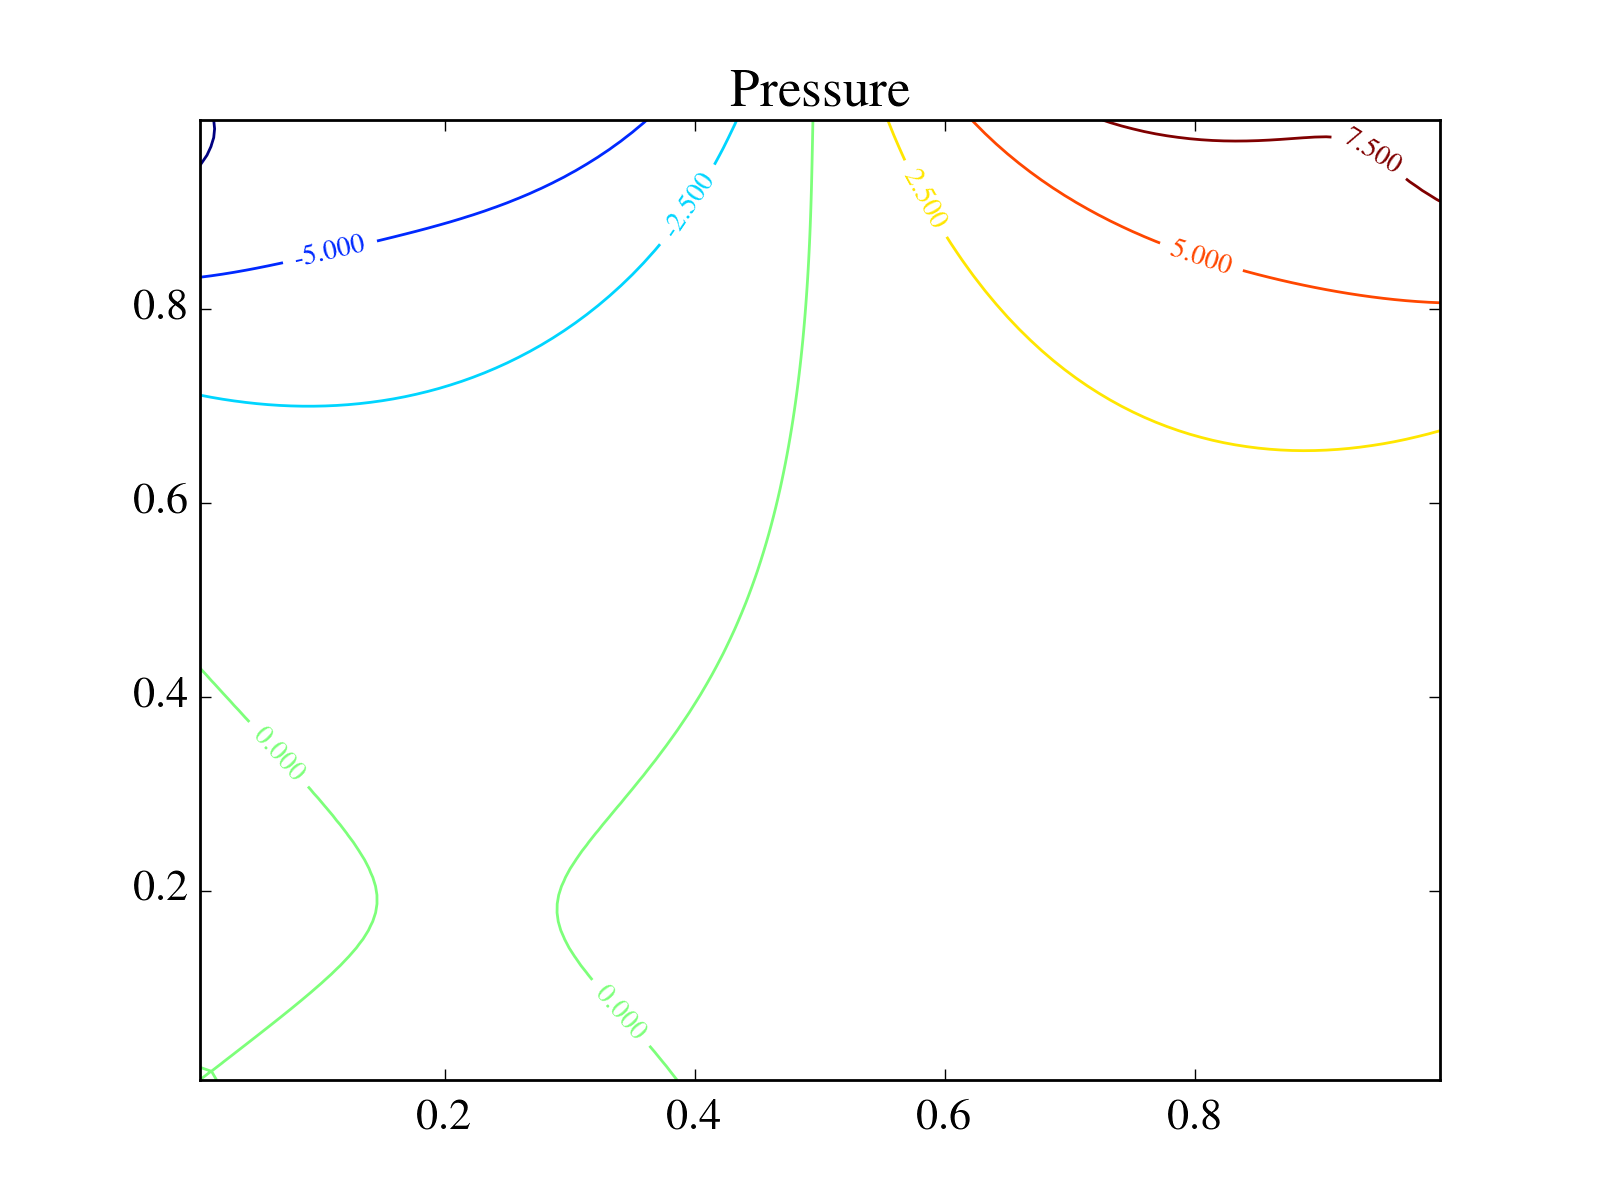
\includegraphics[width=\linewidth]{figures/Re001/n/pressure}
\caption{Contour plot for pressure of the flow in Figure \ref{Re001nVectorField}. \label{Re001nPressure}}
\end{figure}

\begin{figure}[!t]
\centering
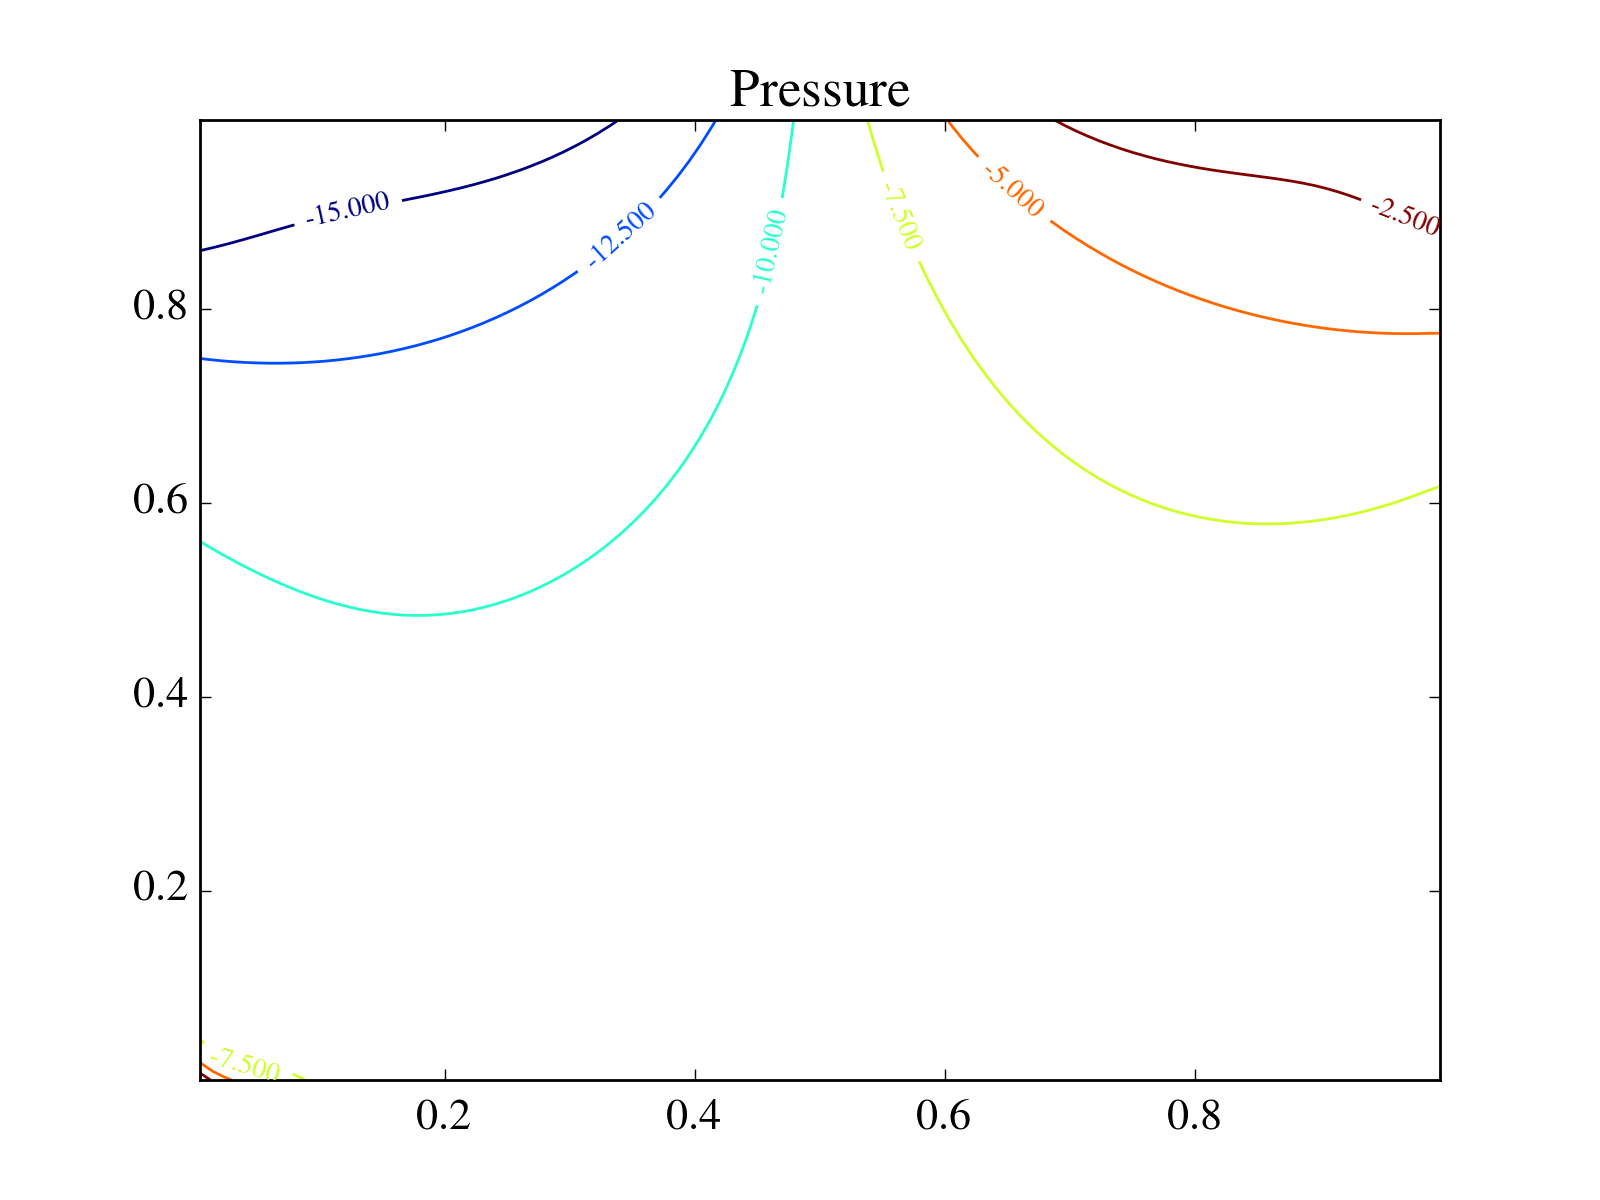
\includegraphics[width=\linewidth]{figures/Re001/w/pressure}
\caption{Contour plot for pressure of the flow in Figure \ref{Re001wVectorField}\label{Re001wPressure}}
\end{figure}



\begin{figure}[!t]
\centering
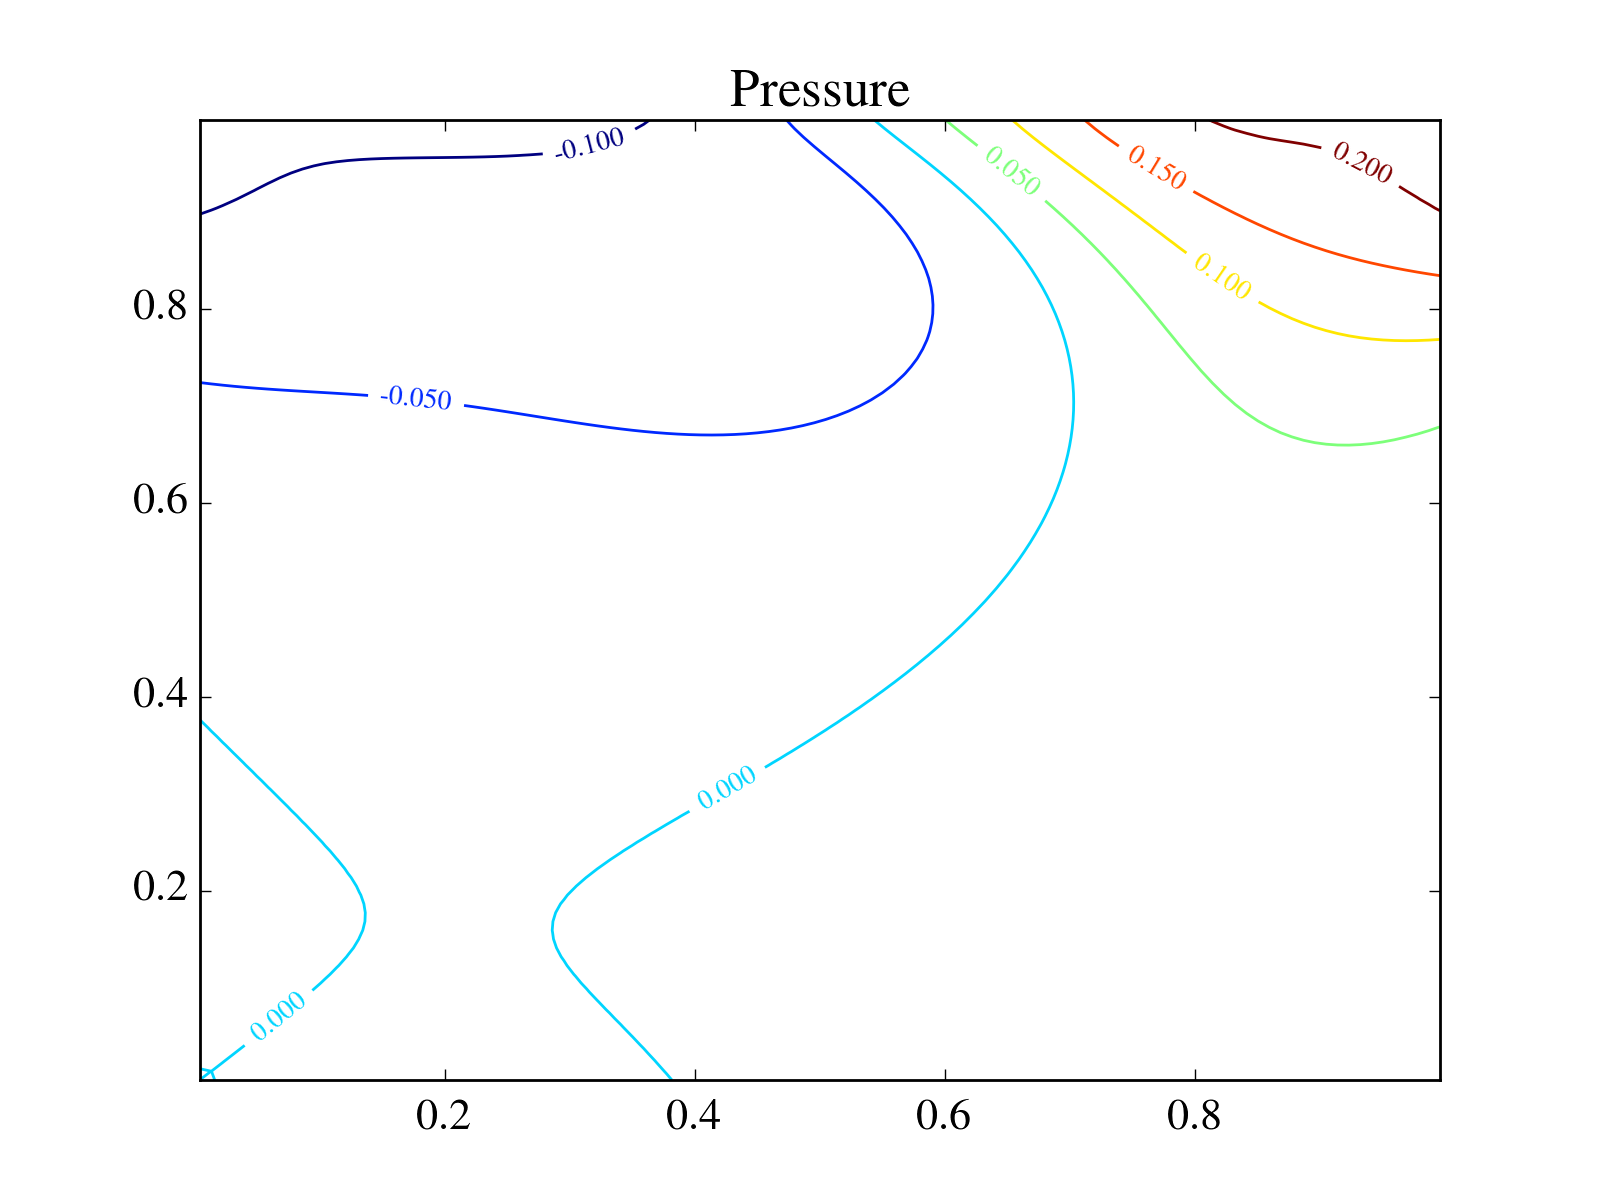
\includegraphics[width=\linewidth]{figures/Re050/n/pressure}
\caption{Contour plot for pressure of the flow in Figure \ref{Re050nVectorField}\label{Re050nPressure}}
\end{figure}


\begin{figure}[!t]
\centering
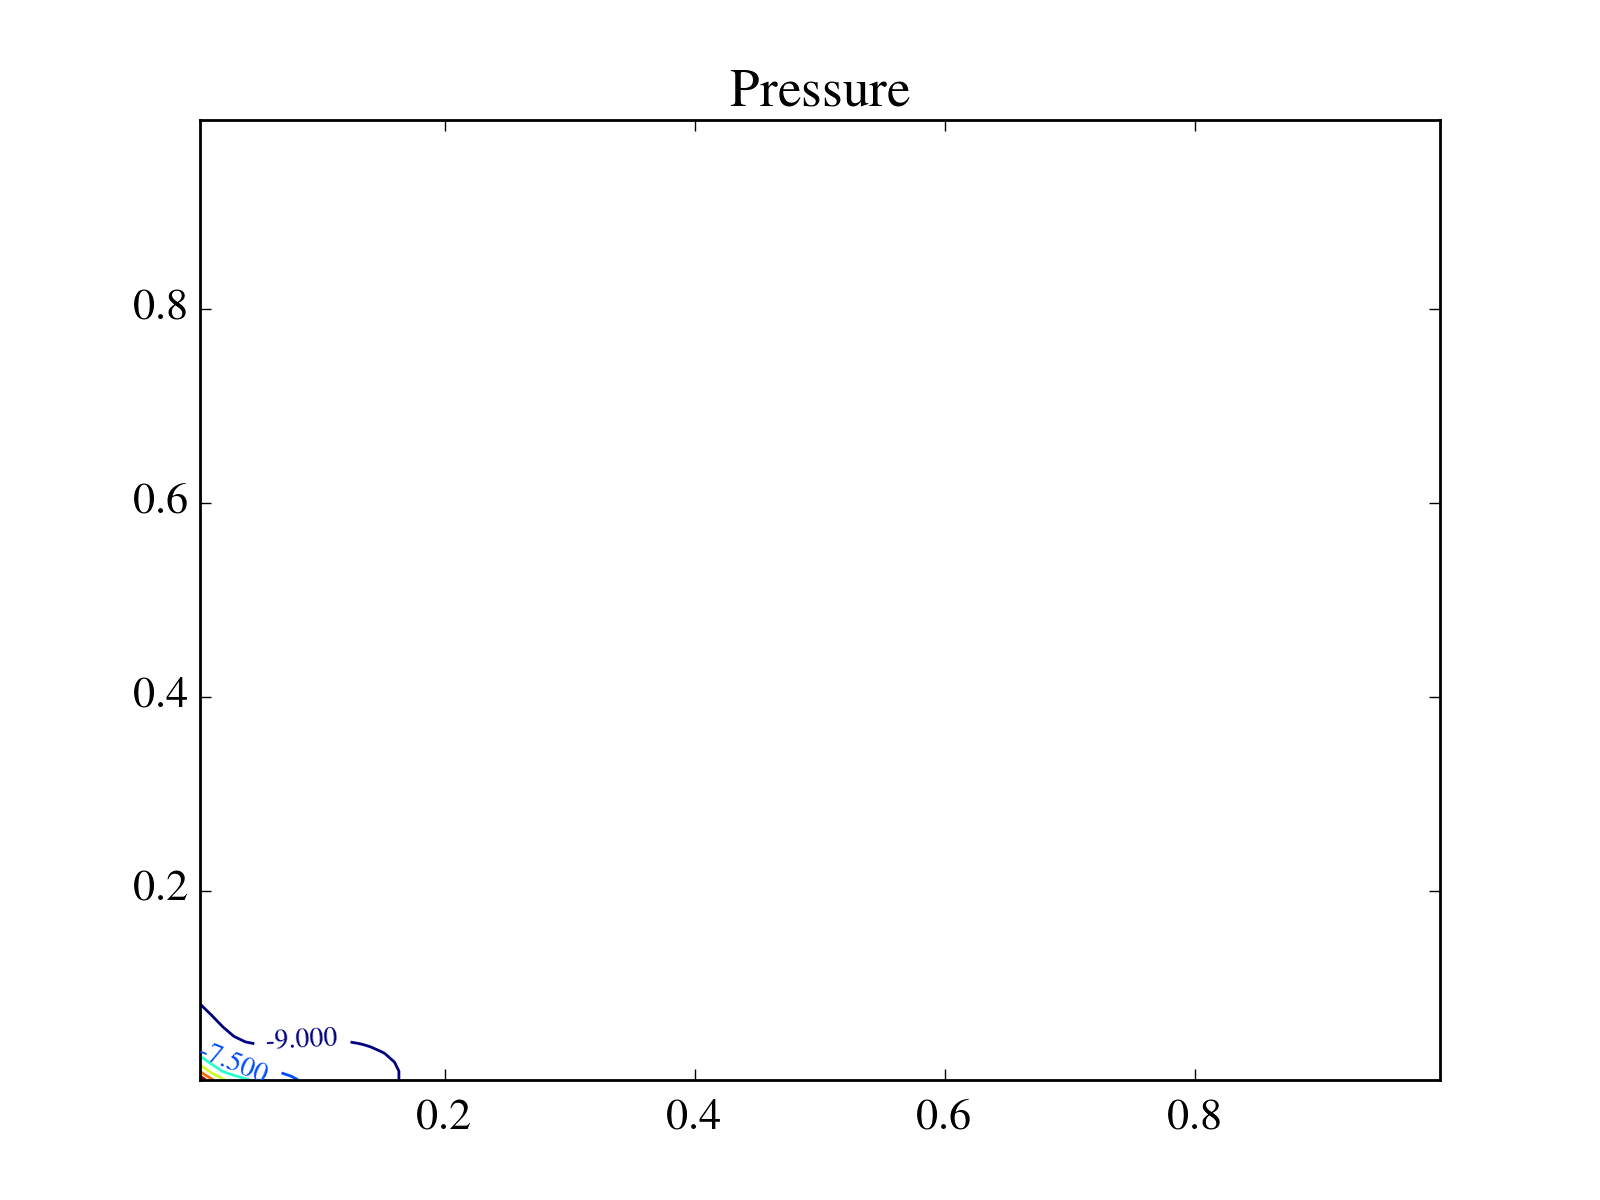
\includegraphics[width=\linewidth]{figures/Re050/w/pressure}
\caption{Contour plot for pressure of the flow in Figure \ref{Re050wVectorField} \label{Re050wPressure}}
\end{figure}



\begin{figure}[!t]
\centering
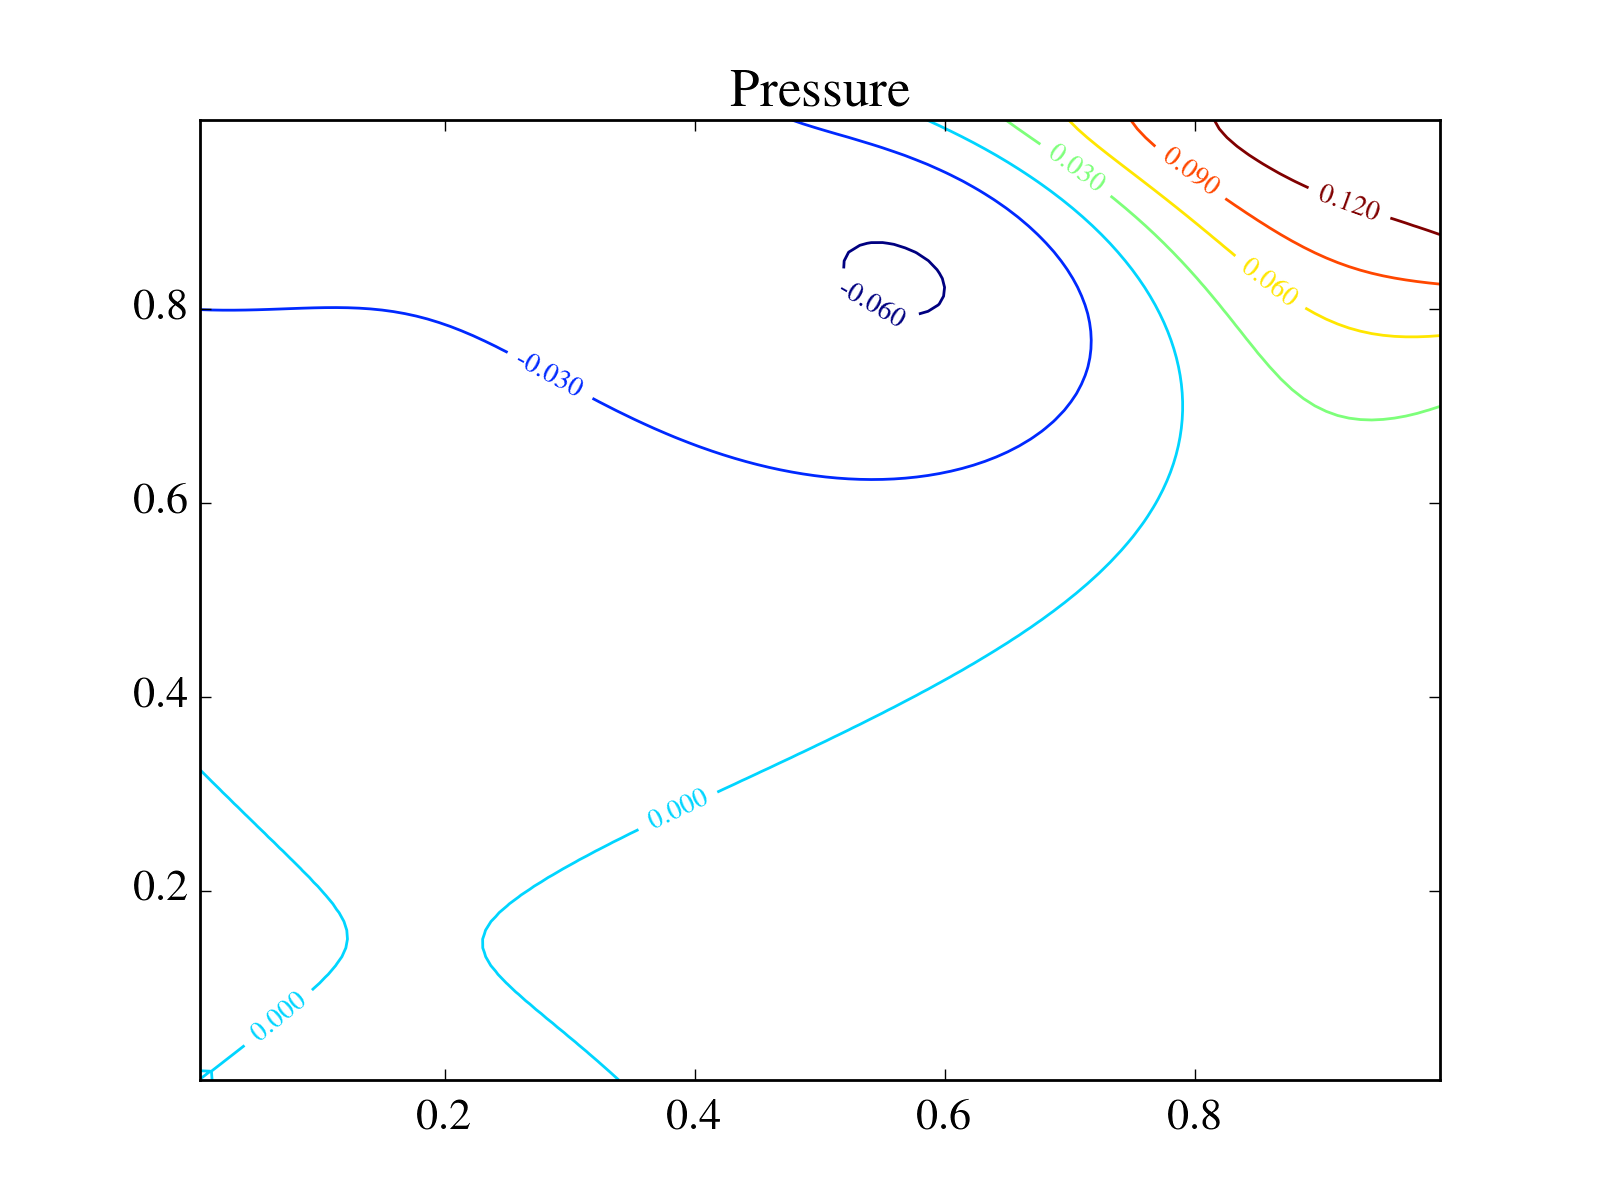
\includegraphics[width=\linewidth]{figures/Re100/n/pressure}
\caption{Contour plot for pressure of the flow in Figure \ref{Re100nVectorField}\label{Re100nPressure}}
\end{figure}


\begin{figure}[!t]
\centering
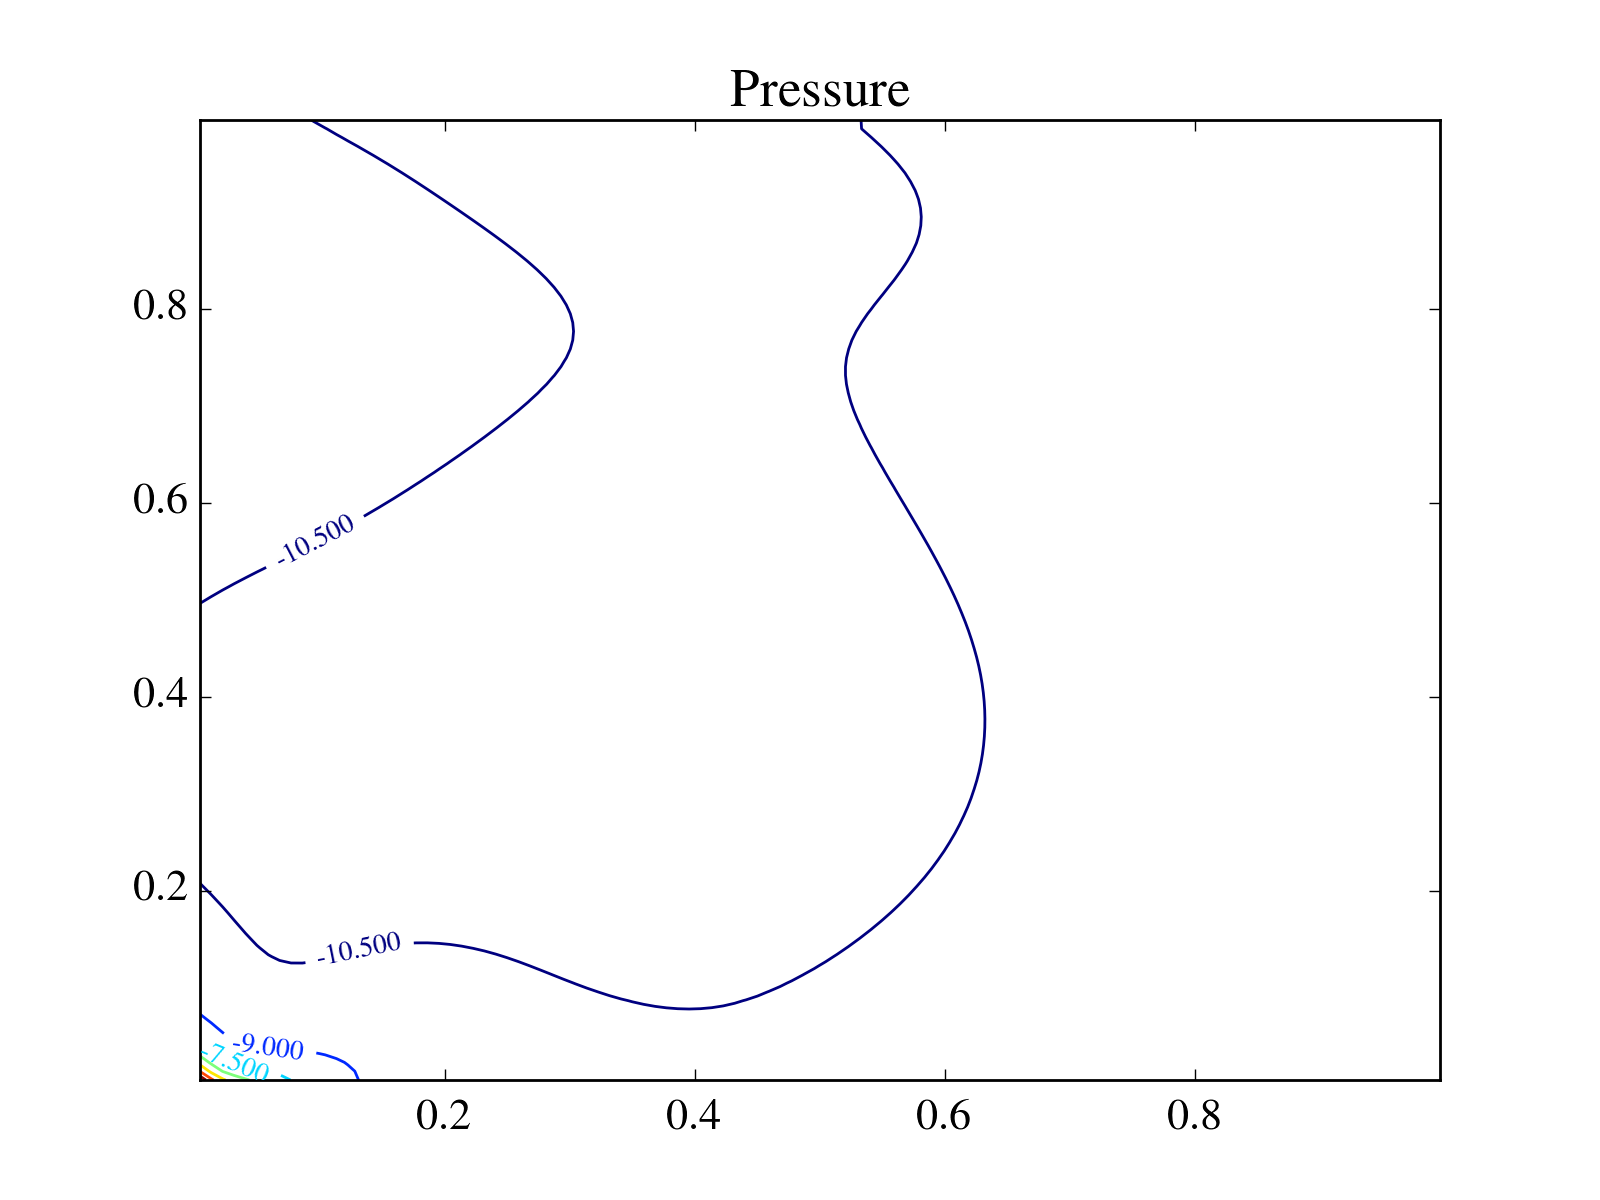
\includegraphics[width=\linewidth]{figures/Re100/w/pressure}
\caption{Contour plot for pressure of the flow in Figure \ref{Re100wVectorField} \label{Re100wPressure}}
\end{figure}

Regarding the results with no magnetic field, Figures \ref{Re001nVectorField} to \ref{Re100nPressure} present very similar results. Although the Reynolds number changes by a factor of 100, no major changes in the steady state flow were able to be observed. It is noticeable, though, that the flow is more asymmetric and the center of the main vortex shifts to the right as $\mathit{Re}$ increases.

This changes dramatically when a magnetic field is in action. A small vortex already appears in Figure \ref{Re001wVectorField} and just grows larger as the Reynolds number increases up to 100 (Figures \ref{Re050wVectorField} and \ref{Re100wVectorField}). Pressure also varies much more and a particular concentration of contour lines is observable close to the origin (the magnetic field is applied just a little off the origin) as presented in Figures \ref{Re001wPressure}, \ref{Re050wPressure} and \ref{Re100wPressure}.


\section{Conclusion}

It is important for the code to be correct, otherwise it is meaningless to analyze the simulation results. The validation step shows that certainly the system is behaving as second order. 

Although not presented in the last sections, it is interesting to observe that one problem that appeared was when physics was disregarded. Trying to apply an arbitrary magnetic field has a good chance of generating results that converge but are incorrect when the governing equations are checked. The results presented comply to the laws that we claim to be following. This is also good evidence of correctness.

This work was a challenge in the aspect that an analytical solution was not available to check against, so it is important to state the importance of the validation step. The results were satisfactory and the tools here coded for exploring magnetic fluids are starting to get usable, when compared with the stage of one year ago.


\section{Future work}
The results presented do not include Reynolds greater than 100 because the code is not currently abiding by any upwind scheme. This is something that is planned to be implemented. Also, a different magnetic field will be used, particularly the one of a Neodymium magnet, instead of the magnetic field of a wire, as used here.

Most importantly, we want to implement the dynamic evolution equations for the magnetization of the ferrofluid that are coupled with the flow field. This will certainly change significantly the dynamics of the flow and will be the subject of our next project.




\section*{Acknowledgments}

Firstly, I thank God for this opportunity. I appreciate professor Yuri Dumaresq for his orientations so that this work could be done. Also, many thanks to CNPq for the scholarship.


\bibliographystyle{plain}
\bibliography{pibic}


\end{document}
